\documentclass[12pt]{report}

\usepackage{graphicx, color}
\usepackage[utf8]{inputenc}
\usepackage[english]{babel}
\usepackage[a4paper,margin=2cm]{geometry}
\usepackage{booktabs}
\usepackage{hyperref}
\usepackage{amsmath}

\newcommand{\red}[1]{{\color{red}{#1}}}

\begin{document}

% ============================================================
\chapter{Introduction}
% ============================================================

Large language models have become capable agents that can plan, reason, and
call external tools to act in the world~\cite{brown2020gpt3,codeact2024}.
The standard framing of this capability is \emph{tool use}: given a fixed set
of pre-built functions, an agent selects the right one and passes the right
arguments~\cite{schick2023toolformer}. Benchmark suites such as
MCP-Universe~\cite{mcpuniverse2025}, MCPAgentBench~\cite{mcpagentbench2024},
and WAPIIBench~\cite{wapiibench2025} measure this ability extensively,
and the field has made substantial progress on it.

What these benchmarks leave unexamined is the step that must come before tool
use in any realistic deployment: someone has to create the tools in the first
place. In practice this is done by human engineers who read API documentation,
write wrapper code, and expose the result through a protocol the agent can
call. This process does not scale. A modern enterprise ecosystem spans hundreds
of REST APIs; keeping tool wrappers current as those APIs evolve is a
continuous maintenance burden. The gap between the APIs that exist and the APIs
that agents can actually reach is, at present, almost entirely a human-labour
bottleneck.

An appealing alternative is \emph{tool synthesis}: letting the model itself
read documentation and produce the tool implementation. Contemporary models can
write code~\cite{toolfactory2025}, operate as autonomous agents with file-system
access~\cite{codeact2024}, and generate callable tool implementations from
unstructured documentation~\cite{doc2agent2025}.
The combination suggests that producing a functional, deployable tool server
from raw API documentation may already be within reach. Yet no prior work has
systematically evaluated this capability across diverse APIs under controlled
conditions: existing benchmarks either assume tools exist, focus on
single-function code generation without live API execution, or assess
high-level agent behaviour without examining the tool layer at all.

This shift from tool use to tool synthesis is conceptually framed by the
\emph{LLM as Tool Maker} (LATM) paradigm~\cite{cai2023latm}, in which a
capable model acts as an architect that proposes, verifies, and packages
software tools for downstream use. The adoption of the Model Context Protocol
(MCP)~\cite{anthropic2024mcp} makes this practically tractable. Unlike
traditional REST integrations, which require bespoke human-engineered
connectors for each client--API pair, MCP wraps heterogeneous backends in a
uniform JSON-RPC interface that agents can discover and call at runtime. This
collapses integration complexity from $N \times M$ (every model client wired
to every API) to $N + M$ (each side adapts once to the shared protocol),
making automated synthesis the natural path to scaling agentic tool coverage.

A fundamental tension arises, however, at the boundary of neural generation
and software execution. API interfaces are rigid: parameter names must match
exactly, types must be correct, and HTTP payloads must conform to schema.
LLMs generate code and serialise arguments through probabilistic token
selection, which does not inherently respect these hard constraints. More
importantly, the large presence of standardised API patterns and open-source
library code in pre-training corpora creates strong, low-entropy priors over
common software utilities. For well-known APIs such as GitHub or Stripe,
a model may produce a functionally correct wrapper entirely from memory,
ignoring the documentation provided at inference time. This phenomenon ---
sometimes called \emph{parametric gravity}~\cite{mallen2023knowns,juice2025} ---
means that in-context documentation does not automatically override
training-time knowledge, particularly for APIs that are heavily represented
in pre-training data.

These observations motivate a systematic study. This thesis asks: \emph{can language models reliably
synthesize functional API tool servers from documentation, and do those
servers enable effective agent task completion?} To answer this, we introduce
an end-to-end benchmark covering 14 REST APIs drawn from productivity tools,
e-commerce platforms, communication systems, financial services, and developer
tooling. The APIs are chosen to vary along two axes: \emph{familiarity}
(the degree to which the API is likely represented in pre-training data) and
\emph{complexity} (number of endpoints, parameter density, and structural
depth). For each API, a synthesis agent is given raw documentation and asked
to produce a complete, runnable MCP server. The resulting server is then
evaluated by a separate agent that attempts 13--25 natural-language tasks
against it, with outcomes judged by a third language model.

Formally, tool synthesis is an autoregressive generation process conditioned
on a task specification $T$, the model's static weights $\theta$, and an
external documentation context $C$:
%
\begin{equation}
  P(X \mid T, C;\, \theta)
  = \prod_{i=1}^{n} P(x_i \mid x_{<i},\, T,\, C;\, \theta)
  \label{eq:synthesis}
\end{equation}
%
where $X = (x_1, \ldots, x_n)$ is the generated server implementation.
We study three instantiations of the context $C$: the full documentation
$C_{\text{docs}}$, the empty context $C_{\emptyset}$ (no documentation), and
a counterfactually mutated context $C_{\text{mut}}$ in which core parameter
names are renamed to conflict with training-time knowledge. Holding $T$ and
$\theta$ fixed while varying $C$ isolates how much the output distribution
depends on in-context evidence versus the parametric knowledge encoded in
$\theta$.

Beyond feasibility, we use the benchmark to investigate two further questions.
First, to what extent do models rely on \emph{parametric knowledge}---facts
absorbed during pre-training---rather than the documentation provided at
inference time? We study this through three synthesis conditions corresponding
to different values of $C$ in Equation~\ref{eq:synthesis}: with full
documentation, without any documentation, and with documentation whose
parameter names have been deliberately mutated to conflict with training-time
knowledge. Mutation adherence is measured at two levels: the Python function
signature (interface layer) and the outbound HTTP payload (network layer),
allowing us to detect where parametric gravity asserts itself during
generation. Second, does synthesis quality predict agent task performance?
We measure synthesis sufficiency separately from end-to-end task execution,
asking whether an LLM judge's assessment of the server --- without running
any tasks --- is a reliable leading indicator of whether the agent will
succeed downstream.

Existing software engineering benchmarks such as SWE-bench~\cite{jimenez2023swebench}
evaluate agents as black boxes, measuring macro pass/fail rates without
explaining where and why failures occur. Conversely, mechanistic work on
parametric memory and context--memory conflict~\cite{mallen2023knowns,longpre2021entity,juice2025}
is largely restricted to open-domain question-answering datasets, which do not
capture the stateful, protocol-driven constraints of live API execution. This
thesis bridges that gap empirically: we measure parametric influence through
controlled documentation ablations and counterfactual mutations, using a live
execution environment as the ground truth signal.

A natural follow-on question is \emph{where in the model} parametric gravity
asserts itself. When a synthesis model ignores a mutated parameter name and
reverts to its training-time prior, this reversal must be traceable to some
point in the forward pass --- a layer at which the residual stream
representation of the in-context token gives way to the attractor encoded in
the model weights~\cite{meng2022rome,factualrecall2025}. We conduct a
preliminary investigation of this question using a log-linear probe on the
residual stream of a smaller open-weight model, examining at which transformer
layers representations of mutated parameter names are overridden by their
training-time counterparts~\cite{alain2017understanding,belrose2023tunedlens}.
This analysis is exploratory and does not constitute a primary empirical
contribution, but it provides a mechanistic grounding for the behavioural
patterns observed in the benchmark and points toward richer explanations of
when and why in-context documentation fails to ground generation.

Beyond empirical analysis, we distil the findings into a set of practical
design guidelines for practitioners building LLM-based tool synthesis systems.
These cover documentation structure and pre-processing, server specification
format, synthesis prompt design, and post-synthesis validation strategies.
While not a formal contribution, these guidelines follow directly from the
failure modes identified in the benchmark and are intended to make the
results actionable for practitioners who need to deploy synthesis pipelines
at scale.

Our main findings are: (i)~synthesis is feasible for most APIs under the
best conditions (median agent pass rate~80\%), and synthesized servers match
or exceed human-authored reference implementations on GitHub and Zulip;
(ii)~removing documentation does not degrade---and sometimes improves---
performance on high-frequency APIs, because model weights already encode
correct implementations and documentation adds context noise;
(iii)~mutation adherence is near-zero for well-known public APIs, confirming
that parametric knowledge dominates documentation for those APIs, and its
effect on agent performance depends on whether both the synthesizer and the
agent share the same prior about the API;
(iv)~synthesis pass rate and agent pass rate are strongly correlated
($r = 0.921$), establishing synthesis quality as a reliable proxy for
downstream utility.
We additionally present a preliminary probing analysis connecting the
observed parametric dominance to representational dynamics in the transformer
residual stream, and derive a set of practical guidelines for robust synthesis
system design.

The remainder of this thesis is organised as follows.
Chapter~\ref{ch:related} surveys related work on tool-use benchmarks,
code generation, parametric knowledge, and autonomous agents.
Chapter~\ref{ch:method} describes the benchmark construction, synthesis
pipeline, evaluation harness, and experimental conditions.
Chapter~\ref{ch:results} presents results structured around the five research
questions.
Chapter~\ref{ch:discussion} interprets the findings in light of prior work,
discusses the parametric gravity mechanism and its practical consequences,
and reflects on the limitations of the study.
Chapter~\ref{ch:conclusion} answers each research question, states the
contribution relative to the identified gap, and identifies directions for
future work.


% ============================================================
\chapter{Related Work}
\label{ch:related}
% ============================================================

\section{Tool Use and Tool Synthesis}

The ability of language models to call external functions has been studied
extensively. Early work established that models can be prompted or fine-tuned
to select tools and format arguments from natural-language
instructions~\cite{schick2023toolformer,qin2023toolbench}. More recent
evaluation suites have scaled this substantially: MCP-Universe~\cite{mcpuniverse2025}
evaluates agents against eleven real-world MCP servers spanning six domains;
MCP-Bench~\cite{mcpbench2025} scales this to 250 tools across twenty APIs
and twenty evaluated models; and MCPAgentBench~\cite{mcpagentbench2024}
benchmarks agent efficiency in tool selection and invocation within the
Model Context Protocol (MCP) ecosystem. Common to all of these
is the assumption that tools already exist: the benchmark provides a pre-built
function library and evaluates how well the agent navigates it. Our work
removes this assumption.

The closest prior work to ours is the \emph{LLM as Tool Maker} (LATM)
framework of Cai et al.~\cite{cai2023latm}, in which a powerful model
generates reusable Python tool implementations that a lighter ``tool user''
model subsequently invokes. The key insight is a separation of concerns:
tool creation is expensive (large model, done once per task class) while
tool use is cheap (smaller model, done many times). Our work extends this
separation to the more demanding setting of REST API integration, where
generated tools must satisfy strict interface contracts enforced by live
external services. LATM evaluates generated tools through auto-generated unit tests on a small
validation sample; we evaluate through end-to-end task execution against
real sandboxed APIs, which catches failures that static analysis cannot ---
such as HTTP parameter mismatches or authentication schema errors.

Concurrent work has begun to close this gap. ToolFactory~\cite{toolfactory2025}
proposes a pipeline that parses heterogeneous, unstructured REST API
documentation and generates callable tool stubs --- explicitly targeting the
setting where formal OpenAPI schemas are unavailable. Doc2Agent~\cite{doc2agent2025}
scales a similar idea, demonstrating that LLMs can produce usable tool
implementations from unstructured documentation across dozens of APIs ---
the closest parallel to our synthesis pipeline. Where these works
focus primarily on synthesis coverage, we additionally evaluate the synthesized
servers end-to-end through agent task execution, measure documentation
grounding, and systematically probe the effect of parametric knowledge
through controlled ablations.

A complementary challenge arises when APIs evolve after the synthesis stage.
Recent work on evolving tool use~\cite{evolvingtoolsiclr2025} employs
Monte Carlo Tree Search to adapt tool invocations when API signatures change
at inference time, framing API evolution as a planning problem. This is
distinct from our setting, where we synthesize the server once per API
version, but it points to the broader challenge of keeping tool infrastructure
current --- the problem that motivates automated synthesis in the first place.

Related work has also explored automated client generation from formal API
specifications such as OpenAPI schemas, but these approaches require
structured machine-readable inputs. In practice, many APIs provide only
Markdown documentation, or provide schemas that are incomplete or misaligned
with actual server behaviour. Our benchmark specifically targets this less
structured setting, using scraped Markdown documentation as the sole
synthesis input, which is closer to the conditions a practitioner faces.

\section{Code Generation}

Classical code-generation benchmarks such as HumanEval~\cite{chen2021codex}
and SWE-bench~\cite{jimenez2023swebench} evaluate against unit tests or static
oracles. These settings share a structural limitation for our purposes: they do
not run generated code against a live external service, so a synthesized API
wrapper that compiles and passes mock tests may silently fail when the real API
rejects its HTTP requests.

Recent 2025 work has begun to study live API execution directly.
WAPIIBench~\cite{wapiibench2025} catalogues the error modes of LLM-generated
API integration code against real services, identifying categories such as
authentication failures, incorrect parameter serialisation, and endpoint
version mismatches. This taxonomy aligns closely with the failure modes we
observe in our synthesis evaluation. RAG-augmented API code
generation~\cite{ragapidocs2025} shows that retrieving relevant documentation
snippets at generation time reduces hallucinated parameters and improves
execution success, suggesting that context grounding is a tractable
intervention even for models with strong parametric priors. When LLMs Lag
Behind~\cite{lagging2025} focuses specifically on faithfulness failures arising
from training-cutoff drift --- cases where the model generates syntactically
correct code that silently targets a deprecated API version, producing errors
that neither compile-time nor unit-test evaluation would catch. Taken together,
these works confirm that live API execution is a qualitatively different
evaluation regime from static code correctness, and that documentation
faithfulness is a first-class concern rather than a secondary one.

\section{Autonomous Agents}

The agent benchmarking landscape spans web navigation (WebArena~\cite{webarena2023}),
computer control (OSWorld~\cite{osworld2024}), and general open-ended
assistance (GAIA~\cite{gaia2023}). These benchmarks treat the agent's
capability to act as the object of study and abstract over the tool
infrastructure. A related line of work examines agents that generate and execute
code to solve tasks~\cite{codeact2024}, but the generated code is typically a
self-contained script rather than a persistent, reusable interface. We study a
complementary question: can an agent produce tool infrastructure that other
agents can then use, and does that infrastructure remain reliable across diverse
APIs and synthesis conditions?

\section{In-Context Learning and Context Faithfulness}

In-context learning (ICL), the ability of large language models to adapt to
new inputs from examples or instructions in the prompt, was systematically
characterised by Brown et al.~\cite{brown2020gpt3}. A common assumption in
the software engineering community is that supplying live API documentation
in the context window grounds the model's output, ensuring that generated
code reflects the current API specification rather than stale parametric
memory. Subsequent work has complicated this assumption in several ways.

Liu et al.~\cite{liu2023lostmiddle} demonstrated that recall follows a
U-shaped curve across context position: performance is highest for information
near the beginning or end of the context and lowest for information placed in
the middle. For tool synthesis over long documentation files, this implies
that endpoints described in the middle of a document may be systematically
under-represented in the generated server --- a structural bias independent
of parametric knowledge effects. More recent work on disentangling recall and reasoning in long
contexts~\cite{disentanglerecall2025} distinguishes between a model's ability
to retrieve information from the context window and its ability to reason over
that information; the two can fail independently. In our setting, synthesis failures attributable to missed documentation ---
where a large API's endpoints are covered only partially --- may
reflect retrieval limitations rather than reasoning failures.

More directly relevant is work on how models handle context that explicitly
contradicts their parametric priors. Xie et al.~\cite{xie2023adaptive}
showed that models can be steered by stated premises even when those premises
are false, while other studies have found the opposite --- models ignoring
contradictory context when their parametric prior is strong. Our mutation
design sits at this intersection: by introducing deliberate conflicts between
in-context documentation and training-time parameter names, we measure which
signal dominates, and for which APIs, providing a controlled analogue to the
natural conflicts that arise when API documentation evolves after a model's
training cutoff.

A 2025 study on task-dependent conflict resolution~\cite{taskmatters2025}
finds that the degree to which a model defers to context versus its
parametric prior depends not only on entity frequency but also on the
nature of the downstream task: models are more likely to update on
context when the task is procedural rather than factual. This is
directly relevant to tool synthesis, where the model must not merely
recall a parameter name but correctly propagate it through the generated
code --- a procedural constraint that might be expected to promote
context adherence, yet our results show this is often not the case
for well-known APIs.

\section{Parametric Knowledge and Knowledge Conflicts}

A growing body of work examines how language models resolve conflicts between
information encoded in their weights during pre-training and information
provided in context at inference time. Studies have found that models exhibit
a strong prior towards their training distribution, sometimes ignoring
counter-factual evidence in the context~\cite{longpre2021entity},
and that this tendency grows stronger as the amount of training exposure to
a topic increases~\cite{mallen2023knowns}.

Mallen et al.~\cite{mallen2023knowns} provide perhaps the most directly
relevant finding: the probability that a model correctly answers a factual
question from parametric memory scales with the log-popularity of the
corresponding entity (measured via Wikipedia page views as a proxy for
pre-training frequency). Rare entities are reliably retrieved from context;
common entities are retrieved from weights even when context is available. For our setting, this predicts that no-docs synthesis
quality should be highest for APIs heavily represented in pre-training
corpora --- exactly what we observe for GitHub and Stripe.
Longpre et al.~\cite{longpre2021entity} studied entity-based knowledge
conflicts in question answering and found that models with stronger parametric
priors are more likely to ignore contradictory context, providing a direct
precursor to our mutation adherence measurement.

This phenomenon has also been studied in question answering settings where
retrieved passages contradict model priors. Neeman et al.~\cite{neeman2022disentqa}
introduce a counterfactual data augmentation approach that trains models to
maintain separate predictions for parametric and contextual answers
simultaneously, improving robustness to knowledge conflicts. The fact that
a specialised training objective is needed to achieve this separation
underscores how strongly parametric priors resist contextual override by
default. This is relevant to our synthesis model comparison, where models
trained under different regimes (GPT-5.2, Sonnet~4.6, Qwen3-Coder) exhibit
markedly different adherence rates to mutated documentation.

More recent 2025 work has sharpened the understanding of when parametric
knowledge yields to context. JuICE~\cite{juice2025} (ICML 2025 Spotlight)
introduces a controlled training objective that suppresses parametric
interference during context-grounded generation, and demonstrates consistent
accuracy gains on conflict-heavy QA benchmarks. Separately, studies on
calibration in RAG pipelines~\cite{ragknowswrong2025} show that models often
fail to signal uncertainty when their parametric prior conflicts with
retrieved evidence, producing confident but incorrect outputs --- a pattern
visible in our synthesis results for cases where the model silently reverts
to training-time parameter names without any warning in its output.

In the tool synthesis setting, parametric gravity creates a measurable
tension: popular APIs such as GitHub and Stripe are extensively represented
in training corpora, so a model may produce a correct wrapper from memory
alone --- or may resist correcting that wrapper when the documentation
specifies something different. We operationalise this tension through
deliberate parameter-name mutations and measure adherence rates at two
levels: the Python interface signature and the outbound HTTP payload.

\section{Mechanistic Interpretability and Probing}

The behavioural evidence from adherence rates raises a mechanistic question:
at which point in the forward pass does parametric memory override in-context
information? Linear probing provides a systematic methodology for
investigating this. Alain and Bengio~\cite{alain2017understanding} demonstrated
that linear classifiers trained on intermediate layer representations reveal
when and where concepts become linearly decodable across the network's depth,
treating each layer's activation as a probe target. Applied to transformer
language models, this technique has been used to track the emergence of
syntactic and semantic structure across layers~\cite{tenney2019bert}.

The logit lens~\cite{nostalgebraist2020logitlens} extends this idea directly: by
projecting intermediate residual stream states through the model's unembedding
matrix at each layer, it is possible to read off the model's evolving
prediction, revealing how token probabilities develop from early to late
layers. Belrose et al.~\cite{belrose2023tunedlens} refined this into the
tuned lens, training a learned affine transformation per layer to improve the
quality of intermediate predictions. These tools make it possible to detect
at which layer a model's prediction transitions from an in-context
representation to a parametric one.

Meng et al.~\cite{meng2022rome} localised factual recall in GPT-style models
to specific middle-layer MLP modules, finding that factual associations are
stored as a form of key-value memory in feed-forward layers. This provides a
candidate mechanistic account of parametric gravity: in-context
representations of mutated parameter names may compete with these stored
associations at the feed-forward layer where the expected parameter name
is ``looked up.''

Recent 2025 work has refined this picture further.
Factual recall via associative memories~\cite{factualrecall2025} (ICLR 2025
Spotlight) models factual associations in transformers as Hopfield-style
attractor networks encoded in feed-forward MLP weights, providing a
principled account of why well-known entities are resilient to context
override. Post-training reshapes representations~\cite{posttrainingreshapes2025}
(COLM 2025) demonstrates that instruction fine-tuning and RLHF alter the
geometry of the residual stream in ways that affect how strongly parametric
associations resist contextual updates --- a finding relevant to our
observation that different fine-tuned models (GPT-5.2, Sonnet~4.6)
show markedly different adherence rates despite comparable parametric
exposure to the GitHub API.

Our probing analysis uses a log-linear classifier on the
residual stream at each layer to detect the point at which representations
of mutated parameter names diverge from their training-time counterparts,
connecting the behavioural adherence results to this mechanistic literature.

\section{The Model Context Protocol}

The Model Context Protocol (MCP)~\cite{anthropic2024mcp} is an open standard
introduced in 2024 that defines how agents discover and invoke tools exposed
by external servers over a stdio transport. An MCP server exposes a
\texttt{list\_tools()} endpoint that returns typed tool schemas and a
\texttt{call\_tool()} endpoint for invocation. The protocol has seen rapid
adoption across agent frameworks, making it a natural target for automated
tool synthesis. Our benchmark uses MCP as the interface layer between the
synthesized server and the evaluation agent.

MCP-Universe~\cite{mcpuniverse2025} evaluates agents against a curated
collection of real-world MCP servers across diverse domains, establishing
baseline performance figures for tool use within the MCP ecosystem.
Doc2Agent~\cite{doc2agent2025} goes a step further and synthesizes
callable tool implementations from unstructured documentation at scale,
demonstrating that automated tool generation is practically viable. Our work builds on this direction by
introducing controlled ablations (no-docs, mutated) and grounding analysis,
allowing us to separate the contribution of documentation from that of
parametric knowledge --- a question neither MCP-Universe nor Doc2Agent
addresses directly.

\section{Summary}

Table~\ref{tab:related} summarises the positioning of our work relative to
the benchmarks discussed above. The key distinguishing feature is that we
evaluate the \emph{production} of tool infrastructure from documentation,
combined with live API execution, rather than the \emph{use} of pre-existing
tools or the generation of code evaluated against static tests.

\begin{table}[h]
\centering
\small
\caption{Positioning relative to prior benchmarks. \emph{Doc faithfulness}:
measures whether generated output is grounded in provided documentation.
\emph{Mech.\ analysis}: probes internal model representations to explain
observed behaviour.}
\label{tab:related}
\begin{tabular}{lccccc}
\toprule
& \textbf{Tool use} & \textbf{Tool synthesis} & \textbf{Live API}
& \textbf{Doc faithfulness} & \textbf{Mech.\ analysis} \\
\midrule
ToolBench        & \checkmark &            &            &            & \\
API-Bank         & \checkmark &            &            &            & \\
LATM             &            & \checkmark &            &            & \\
HumanEval        &            & \checkmark &            &            & \\
SWE-bench        &            & \checkmark &            &            & \\
MCPAgentBench    & \checkmark &            &            &            & \\
MCP-Universe     & \checkmark &            &            &            & \\
GAIA / WebArena  & \checkmark &            &            &            & \\
ToolFactory      &            & \checkmark &            & \checkmark & \\
Doc2Agent        &            & \checkmark & \checkmark &            & \\
WAPIIBench       & \checkmark &            & \checkmark & \checkmark & \\
MCP-Bench        & \checkmark &            & \checkmark &            & \\
\textbf{Ours}    & \checkmark & \checkmark & \checkmark & \checkmark & \checkmark \\
\bottomrule
\end{tabular}
\end{table}


% ============================================================
\chapter{Methodology}
\label{ch:method}
% ============================================================

\section{Overview}

Our benchmark evaluates tool synthesis end-to-end: a synthesis agent reads API
documentation and produces an MCP server; a separate evaluation agent attempts
natural-language tasks against that server; an LLM judge scores each attempt.
The three-stage design cleanly separates synthesis quality from agent reasoning
ability, allowing failures to be attributed to the correct component. The
process is fully automated and requires no human annotation beyond the initial
task authoring. Figure~\ref{fig:pipeline} illustrates the pipeline.

\begin{figure}[h]
\centering
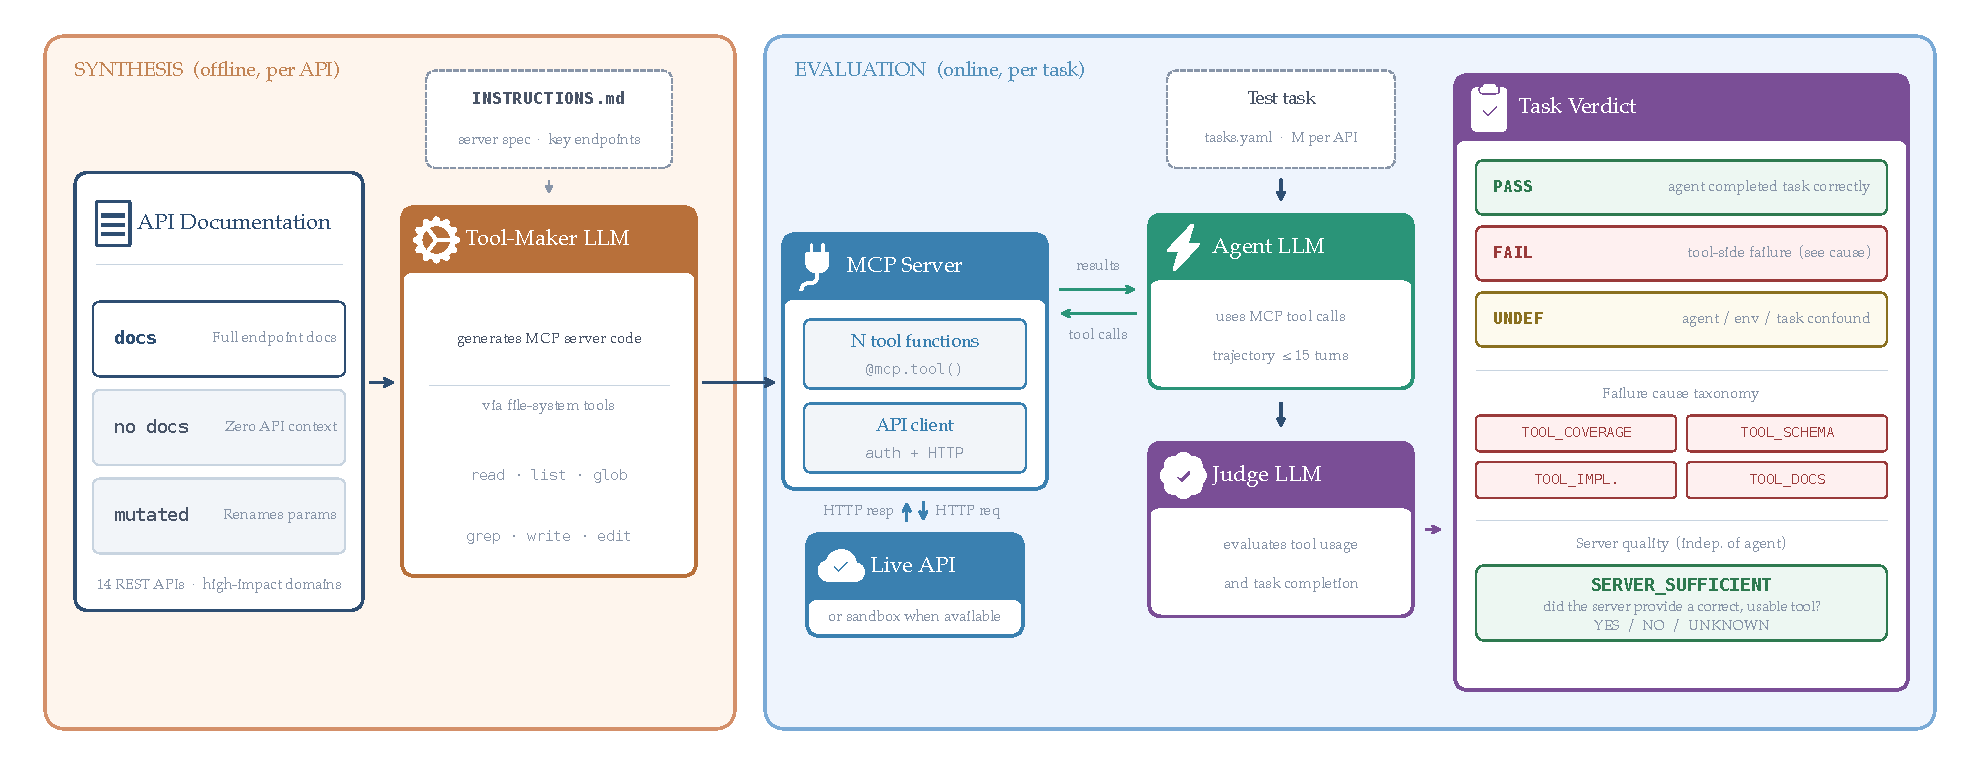
\includegraphics[width=\linewidth]{benchmark_pipeline_thesis_v4.pdf}
\caption{End-to-end benchmark pipeline. A synthesis agent reads documentation
and produces an MCP server; a separate evaluation agent attempts tasks against
it; a judge scores each attempt.}
\label{fig:pipeline}
\end{figure}

\noindent
This separation is the central design choice. In prior tool-use evaluations,
the tool layer is given; here it is produced under test. A synthesized server
that crashes, exposes incomplete tool coverage, or maps arguments incorrectly
will cause agent failures regardless of how capable the evaluation model is.
By isolating the synthesis stage, we can attribute failures to either the
tool infrastructure (synthesis failures) or the evaluation agent (reasoning
failures), and measure how tightly the two are coupled.

\section{Benchmark Datasets}

\subsection{API Selection}

We select 14 REST APIs spanning five domains: developer tooling (GitHub),
productivity and collaboration (Notion, Confluence, Jira), e-commerce
(eBay Buy, eBay Commerce, eBay Sell, Shopify), communication (Mastodon,
Zulip), and data and financial services (Stripe, Alphavantage, Spoonacular,
OpenWeatherMap). Selection criteria were: (i)~availability of a sandboxed or
resettable test environment with stable test credentials, (ii)~REST-based
HTTP interface returning JSON, (iii)~public developer documentation available
as HTML or Markdown, and (iv)~variation along the two primary experimental
axes: \emph{familiarity} (the degree to which an API is likely
well-represented in pre-training corpora) and \emph{complexity} (endpoint
count, parameter density, and authentication complexity).

APIs range from high-familiarity, high-complexity (GitHub, Stripe) to
low-familiarity, low-complexity (Alphavantage, OpenWeatherMap). The eBay
suite provides three difficulty tiers within a single platform: the Buy,
Commerce, and Sell sub-APIs differ substantially in documentation volume and
endpoint coverage despite sharing the same host and OAuth model. Jira and
the eBay Sell API represent the most challenging synthesis targets, with large
hierarchical documentation and high parameter cardinality.

\subsection{Documentation Collection}

For each API, we scrape the official developer documentation portal and convert
it to Markdown using a DOM-to-Markdown pipeline. Depending on the API's
documentation structure, this produces between 7 and 190 Markdown files per
dataset (median approximately 35 files). Files range from single-endpoint
reference pages to category-level overview pages covering multiple related
endpoints. We do not post-process or selectively filter the scraped content
beyond format normalisation; the synthesizer receives the documentation in the
same form it appears online, including navigation artefacts, code samples in
multiple languages, and pagination boilerplate.

This choice is deliberate: it reflects realistic synthesis conditions, where
a practitioner points a synthesis agent at a raw documentation URL rather than
a curated, cleaned API description. The resulting noise is part of the
synthesis challenge the model must handle.

\subsection{Human Reference Servers}

For two APIs --- GitHub and Zulip --- publicly available, community-maintained
MCP servers exist and can be evaluated against the same task suite. The GitHub
MCP server is the official implementation maintained by GitHub; the Zulip
server is a community-contributed open-source project. Both are written in
TypeScript using the official MCP SDK and expose a subset of the respective
APIs as tools. We run both reference servers against the same evaluation agent
and judge pipeline used for the synthesized servers, without any modification.

These human-authored servers serve as a practical baseline: they represent
what a developer with API familiarity and access to the official documentation
would produce without time pressure from an automated benchmark. Crucially,
neither server was constructed with our specific evaluation tasks in mind, so
coverage gaps reflect genuine tool-design choices rather than benchmark
overfitting. Comparing synthesized server PASS rates against these baselines
directly answers whether automated synthesis can match or exceed hand-crafted
implementations (Section~\ref{sec:rq2}).

\subsection{Parameter Mutations}

To probe the degree to which synthesis models rely on parametric knowledge
rather than the provided documentation, we introduce a \emph{mutated}
condition ($C_{\text{mut}}$) for each API. For each dataset, we identify
4--6 core parameter names that are prominent in the API and likely encoded
in training-time weights (e.g.\ \texttt{limit}, \texttt{offset}, \texttt{sort}
for eBay Buy) and replace them uniformly throughout the documentation with
plausible but distinct alternatives (e.g.\ \texttt{max\_results},
\texttt{skip}, \texttt{order\_by}). Replacement names are chosen to be
syntactically plausible --- consistent with conventions in adjacent APIs ---
while being clearly different from the originals at the string level.

A synthesis model that faithfully follows the mutated documentation should
produce tools using the new parameter names consistently. A model dominated
by parametric memory will reproduce the original names regardless. We
quantify this as \emph{mutation adherence}, measured at two levels:

\begin{itemize}
  \item \textbf{Interface adherence}: the mutated name appears as a Python
    identifier in the MCP tool function signature, i.e.\ the evaluation agent
    sees and receives the renamed parameter.
  \item \textbf{HTTP adherence}: the mutated name appears as a quoted string
    key in the outbound HTTP request. This is a stricter criterion; a model
    may adopt the renamed identifier locally but revert to the original name
    when constructing the HTTP payload.
\end{itemize}

\noindent
HTTP adherence is always $\leq$ interface adherence. The gap between the two
is informative: a large gap indicates the model partially follows documentation
(adopting Python argument names) but reverts to training priors when
constructing HTTP calls.

To enable fair PASS comparison across conditions, we apply a \emph{patch}
step to mutated servers before evaluation: the original parameter names are
restored in the source files, so the evaluation agent always calls the real
API with the correct parameters regardless of whether the synthesizer adopted
the mutations. Adherence is measured before patching; PASS is measured after.

\section{Synthesis Pipeline}

\subsection{Task Specification}

Each dataset includes a \texttt{TASK.md} file that provides the synthesis
agent with all information needed to produce a functional server. The
specification covers: the target implementation framework (FastMCP for Python,
or the official \texttt{@modelcontextprotocol/sdk} for TypeScript), the list
of available documentation files and their location, required environment
variables (API keys, OAuth credentials, sandbox flags), authentication flow
(typically OAuth~2.0 client credentials or a static API key), coverage
expectations (broad CRUD on core resource types, support for multi-step
workflows), and required deliverables.

Deliverables are uniform across all datasets and language choices:
\begin{itemize}
  \item \texttt{server.py} (or \texttt{server.ts}): the MCP entry point that
    registers all tools and starts the stdio server.
  \item \texttt{requirements.txt} (or \texttt{package.json}): pinned
    dependencies for reproducible installation.
  \item \texttt{grounding.json}: a manifest mapping every synthesized tool
    name to the source documentation file and HTTP endpoint it implements
    (e.g.\ \texttt{\{"doc": "docs/browse.md", "endpoint":
    "GET /buy/browse/v1/item\_summary/search"\}}).
\end{itemize}

\noindent
The grounding manifest enables two lightweight analyses. \emph{Citation
validity} checks that each entry's \texttt{doc} field names a file that
exists in the documentation corpus and that the \texttt{endpoint} field
contains a syntactically plausible HTTP method--path string. \emph{Grounding
coverage} checks that every synthesized tool has a corresponding entry ---
i.e.\ the synthesizer claimed a source for each tool it produced. These
checks do not verify that the implementation is faithful to the cited
documentation, only that the synthesizer anchored each tool to \emph{some}
real document and endpoint rather than producing an entry-free, free-form
stub.

\subsection{Synthesis Agent}

The synthesis agent operates in an agentic loop with access to a set of
file-system tools. The primary synthesis models (GPT-5.2, GPT-5.4, and
Qwen3-Coder-Next via vLLM) are provided six tools: \texttt{read\_file},
\texttt{write\_file}, \texttt{edit\_file}, \texttt{glob}, \texttt{grep},
and \texttt{list\_directory}. The agent receives the task specification and,
depending on the synthesis condition, a populated documentation directory.
It iterates freely until it produces the required deliverables.

A typical synthesis run follows three phases. In the \emph{exploration} phase
(turns 1--3), the agent reads \texttt{TASK.md}, lists the documentation
directory, and reads a subset of files to understand the API's structure and
authentication model. In the \emph{implementation} phase (turns 4--20), it
writes tool modules and a shared HTTP client. In the \emph{finalisation}
phase (last 2--3 turns), it assembles \texttt{server.py}, writes
\texttt{grounding.json} and \texttt{requirements.txt}, then performs a
self-verification pass by rereading key files. Figure~\ref{fig:synth-trace}
shows a representative trace.

\begin{figure}[h]
\centering
\small
\begin{verbatim}
[turn 1]  read_file(TASK.md)
[turn 1]  glob(docs/*.md)
[turn 2]  read_file(docs/browse.md)
[turn 2]  read_file(docs/item.md)
[turn 4]  write_file(generated_tools/browse.py)
[turn 7]  write_file(generated_tools/order.py)
[turn 9]  write_file(server.py)
[turn 10] write_file(grounding.json)
[turn 11] write_file(requirements.txt)
\end{verbatim}
\caption{Typical synthesis agent trace (eBay Buy, docs condition, GPT-5.2).
813K input tokens, 11K output tokens, 190 seconds.}
\label{fig:synth-trace}
\end{figure}

\noindent
GPT-class synthesizers tend to produce a two-layer architecture: a
\texttt{generated\_tools/} directory of domain-specific Python modules
(e.g.\ \texttt{issues.py}, \texttt{pulls.py} for GitHub), each implementing
a group of related endpoints through a shared HTTP client, with
\texttt{server.py} acting as a thin registration layer applying
\texttt{@mcp.tool()} decorators. Qwen3-Coder-Next typically produces a flat
structure with all tool logic in a single \texttt{server.py}. Both patterns
are accepted by the evaluation harness; only the MCP interface contract
matters for evaluation.

\subsection{Synthesis Conditions}

We evaluate each API under three synthesis conditions, corresponding to three
instantiations of the context $C$ in Equation~\ref{eq:synthesis}:

\begin{itemize}
  \item $C_{\text{docs}}$ \textbf{(with docs)}: the agent receives all
    scraped documentation files in addition to the task specification.
  \item $C_{\emptyset}$ \textbf{(no docs)}: the agent receives only the
    task specification, with no documentation. All tool implementations must
    come from parametric knowledge.
  \item $C_{\text{mut}}$ \textbf{(mutated docs)}: the agent receives the
    mutated documentation, creating a controlled conflict between in-context
    parameter names and training-time priors.
\end{itemize}

\noindent
Synthesis resource usage varies substantially across conditions. GPT-5.2
docs-condition runs typically require 15--25 agent turns, consuming
14K--2.4M input tokens (reflecting documentation corpus size, which ranges
from 7 to 190 files). No-docs runs are substantially shorter: 14K--24K input
tokens and approximately 1 minute wall time, since the agent skips document
reads and writes directly from parametric memory.

\subsection{Synthesis Models}

We evaluate five synthesis models. GPT-5.2 serves as the primary baseline,
run across all 14 APIs and all three conditions. GPT-5.4 is run across all
14 APIs as a more recent baseline. Sonnet~4.6 (Claude Sonnet) is run across
a representative subset of APIs. Gemini~3.1~Pro provides a third model family
for comparison. Qwen3-Coder-Next is run locally via a vLLM inference server.
These span a range of training corpora, post-training regimes, and context
window sizes, allowing us to assess whether synthesis quality is model-specific
or reflects a more general capability. Model comparison results are presented
in Section~\ref{sec:rq1}.

\section{Evaluation Framework}

\subsection{Evaluation Tasks}

For the 14 APIs in the primary evaluation set, we manually authored 13--25
natural-language tasks per API (265 tasks total; median 19 per API). Tasks
are specified in a \texttt{tasks.yaml} file using a four-field schema:

\begin{verbatim}
- id: search_products
  prompt: >
    Search for "wireless headphones" on eBay. Report the title,
    price, and item ID of the first 5 results.
  expected: itemId
  tags: [read]
\end{verbatim}

\noindent
Tasks follow four design principles. First, prompts are \emph{goal-oriented}:
they describe the desired outcome without naming tools, parameter fields, or
HTTP endpoints. Second, they provide only the domain knowledge the agent
cannot infer from tool schemas (e.g.\ ``amounts are in cents''), not call
sequences or parameter names. Third, they require \emph{synthesis over echo}:
comparison, counting, filtering, or multi-step retrieval rather than raw
response reporting. Fourth, chain depth is capped at six sequentially
dependent calls, with the intended range being 2--4 steps.

The \texttt{expected} field contains a task-specific substring --- typically
a field name, ID, or derived value --- that can only appear in the agent's
final answer if it called the correct tool with semantically correct
parameters. This string is passed to the judge as a ground-truth hint,
reducing ambiguity in open-ended response scoring.

Tasks are distributed across four functional categories: smoke tests
(single-call reads verifying basic tool reachability), multi-step workflows
(search then retrieve, create then verify), error-handling tasks (invalid IDs,
missing resources, permission boundaries), and harder synthesis tasks
requiring pagination, cross-resource joins, or derived computations. Write
tasks use a consistent naming prefix (e.g.\ \texttt{"Agent Eval Test *"})
to facilitate cleanup and prevent cross-run contamination.

\subsection{Evaluation Agent}

The evaluation agent (Gemini~2.5~Pro) connects to the synthesized MCP server
via stdio transport and executes an agentic loop. At each turn it receives the
full message history --- system prompt, task prompt, and all prior tool results
as \texttt{ToolMessage} objects --- and responds with either a set of tool
calls or a final textual answer. The loop terminates when the model emits a
response with no tool calls, or after a maximum of 15 turns.

The agent's system prompt instructs it to always call at least one tool before
answering, use observed tool results to inform subsequent calls, and pass
environment-specific constants (e.g.\ \texttt{EBAY\_ENVIRONMENT=SANDBOX})
verbatim rather than inferring them. The prompt does not describe individual
tools or their signatures; the agent discovers available tools at runtime by
calling \texttt{list\_tools()}. The agent does not perform explicit chain-of-thought
reasoning steps between tool calls; reasoning is implicit in the model's
generation.

The evaluation harness speaks only MCP: it calls \texttt{list\_tools()} to
discover available tools and \texttt{call\_tool(name, args)} to invoke them.
No other protocol or API client is provided. All HTTP logic --- authentication,
request construction, token refresh, error handling --- executes inside the
synthesized server process and is invisible to both the harness and the
evaluation agent. The evaluation agent's performance therefore depends entirely
on the interface quality and implementation correctness of the synthesized server.

\subsection{Judge}

Task outcomes are assessed by a separate LLM judge (Gemini~3~Flash) that
does not participate in the agentic loop. The judge receives a structured
prompt containing four components: the original task prompt, the list of all
tool names and their one-line descriptions (from \texttt{list\_tools()}),
the full tool-call trajectory formatted as numbered steps
(\texttt{Step N: tool\_name(\{args\}) $\rightarrow$ [truncated result]}),
and the agent's final textual answer. It is asked three questions:

\begin{enumerate}
  \item \textbf{OUTCOME}: Did the agent complete the task correctly?
    (\textsc{pass} / \textsc{fail})
  \item \textbf{FAILURE\_CAUSE}: If \textsc{fail}, what was the primary cause?
    One of eight codes:
    \textsc{tool\_coverage} (required tool absent from server),
    \textsc{tool\_documentation} (tool present but name or description
    prevented the agent from identifying it),
    \textsc{tool\_schema} (tool present but parameters incorrectly typed
    or named),
    \textsc{tool\_implementation} (tool called correctly but returned wrong
    or malformed data),
    \textsc{agent\_reasoning} (tools were sufficient but agent misused them),
    \textsc{task\_ambiguous} (task wording unclear or contradictory),
    \textsc{environment} (server crash, network error, credential failure),
    \textsc{none} (used when \textsc{outcome} is \textsc{pass}).
  \item \textbf{SERVER\_SUFFICIENT}: Setting aside what the agent did,
    did the synthesized server provide all tools needed to complete the task?
    (\textsc{yes} / \textsc{no} / \textsc{unknown})
\end{enumerate}

\noindent
The judge responds in a fixed plain-text format (no markdown) to enable
reliable parsing:

\begin{verbatim}
OUTCOME: PASS
FAILURE_CAUSE: NONE
SERVER_SUFFICIENT: YES
REASON: The agent correctly identified the search tool, applied the
        right filters, and extracted the requested itemId values.
\end{verbatim}

\noindent
The \textsc{tool\_documentation} category distinguishes a missing tool
(coverage gap) from a present-but-undiscoverable tool (documentation gap):
when the server implements the correct endpoint but gives it a misleading
name or description, the agent fails not because the tool is absent but
because it cannot identify it. This distinction is absent from most prior
tool-use benchmarks and matters for understanding where synthesis quality
breaks down independent of coverage.

\subsection{Metrics}
\label{sec:metrics}

We report two primary metrics derived from the judge's structured output.

\textbf{PASS} is the fraction of task attempts scored \textsc{pass} out of
all \emph{scoreable} attempts. A task attempt is excluded from the denominator
if it is attributed to \textsc{environment} (external infrastructure failure
unrelated to synthesis quality) or \textsc{task\_ambiguous} (measurement
confound). Failures attributed to \textsc{agent\_reasoning} are also excluded:
they count neither as pass nor fail, because they reflect the evaluation
agent's behaviour rather than the synthesized server. PASS is thus a clean
signal about tool infrastructure quality:
%
\begin{equation}
  \text{PASS}
  = \frac{\#\,\textsc{pass}}
    {\#\,\textsc{pass} + \#\,\textsc{fail}_{\text{tool}}}
  \label{eq:pass}
\end{equation}
%
where $\#\,\textsc{fail}_{\text{tool}}$ counts failures attributed to
\textsc{tool\_coverage}, \textsc{tool\_documentation},
\textsc{tool\_schema}, or \textsc{tool\_implementation}.

\textbf{SYNTH} (synthesis sufficiency) is derived from the
\textsc{server\_sufficient} verdict: it is the fraction of tasks for which
the judge found the server sufficient regardless of whether the agent
succeeded. SYNTH measures synthesis quality independently of the evaluation
agent, and is computed only for tasks where the judge returned a
non-\textsc{unknown} verdict. When SYNTH is high but PASS is low, the
bottleneck is agent reasoning; when both are low, the bottleneck is synthesis.

Together, the two metrics place each API--condition data point in one of
three regimes: \emph{synthesis-limited} (low SYNTH, low PASS),
\emph{agent-limited} (high SYNTH, lower PASS), or \emph{ceiling} (high SYNTH,
high PASS). The scatter plot of SYNTH against PASS (Section~\ref{sec:rq5})
visualises this decomposition across all 42 API--condition pairs in the
primary evaluation.

% ============================================================
\chapter{Results}
\label{ch:results}
% ============================================================

This chapter presents results for the five research questions introduced in
Chapter~\ref{ch:method}. Section~\ref{sec:rq1} establishes that synthesis
is feasible for most APIs. Section~\ref{sec:rq2} shows that synthesized
servers enable effective agent task completion and compares against
human-authored references. Section~\ref{sec:rq3} characterises how
synthesizers rely on parametric knowledge and when this affects downstream
performance. Section~\ref{sec:rq4} examines the effect of documentation
availability. Section~\ref{sec:rq5} quantifies the relationship between
synthesis quality and agent pass rate.

% ------------------------------------------------------------
\section{RQ1: Synthesis Feasibility}
\label{sec:rq1}
% ------------------------------------------------------------

\textbf{Can LLMs synthesize functional API tool servers from documentation alone?}

Figure~\ref{fig:heatmap} shows PASS and SYNTH across all 14 APIs and three
synthesis conditions. Twelve of 14 APIs achieve SYNTH $\geq 75\%$ in the
docs condition, with a median of approximately 84\%. Only Jira (56\%) and
eBay Sell (43\%) fall consistently below that threshold, indicating that
synthesis is feasible for the large majority of APIs tested.

The dominant failure mode is \emph{coverage gap}: the server starts and
runs correctly, but the synthesizer omits the specific endpoints required
by certain benchmark tasks. This is most pronounced for large APIs with many
endpoints (eBay Sell, Jira), consistent with the negative trend between
endpoint count and SYNTH visible in Figure~\ref{fig:complexity}. Structural
failure --- servers that crash or omit the required \texttt{server.py}
entrypoint entirely --- is rare with GPT-5.2 (the primary synthesis model)
and occurs mainly with weaker or smaller models.

A synthesis variance study (5--6 repeated runs per condition for Shopify,
GitHub, and Stripe) reveals that degeneracy rate is condition-dependent.
Shopify docs produces zero degenerate stubs across five runs; GitHub docs
produces degenerate stubs (fewer than five tools) in 4 of 6 runs (67\%);
and GitHub mutated produces degenerate stubs in all 7 additional runs (100\%
degeneracy) --- the mutated grounding document consistently confuses the
synthesizer for this complex API. When valid synths are produced, per-condition
variance is moderate: Shopify docs PASS ranges 59--93\% ($\sigma \approx 13$~pp)
while Shopify nodocs is almost perfectly stable (PASS 80--94\%, SYNTH locked
at 94\% across all five runs with $\sigma = 0$). These variance figures
motivate the use of multiple synthesis candidates per condition in deployment
settings, rather than accepting a single synthesis run.

SYNTH is notably stable across conditions for most APIs: Confluence holds
at 95\% across all three conditions and Mastodon at 93--100\%, indicating
that synthesis quality is primarily determined by API structure rather than
what context is provided. The exceptions --- eBay Commerce drops from
SYNTH=100\% (docs) to 54\% (mutated) --- arise where parameter mutations
reduce tool coverage directly.

Grounding analysis shows that synthesizers consistently anchor tools to
real documentation sources: citation validity is 86--100\% across datasets
(every \texttt{grounding.json} entry points to an existing file with a
syntactically plausible endpoint string), and grounding coverage is complete
(every synthesized tool has a corresponding entry). This rules out the
possibility that high SYNTH scores are driven entirely by tools whose
implementations are unmoored from any documentation --- though it does not
verify that each tool correctly implements what its cited document describes. Even in the
no-docs condition, SYNTH remains high for well-known APIs (GitHub nodocs
SYNTH=87\%), suggesting that parametric knowledge can partially substitute
for documentation at the synthesis stage --- a finding developed further in
Section~\ref{sec:rq3}.

\begin{figure}[htbp]
  \centering
  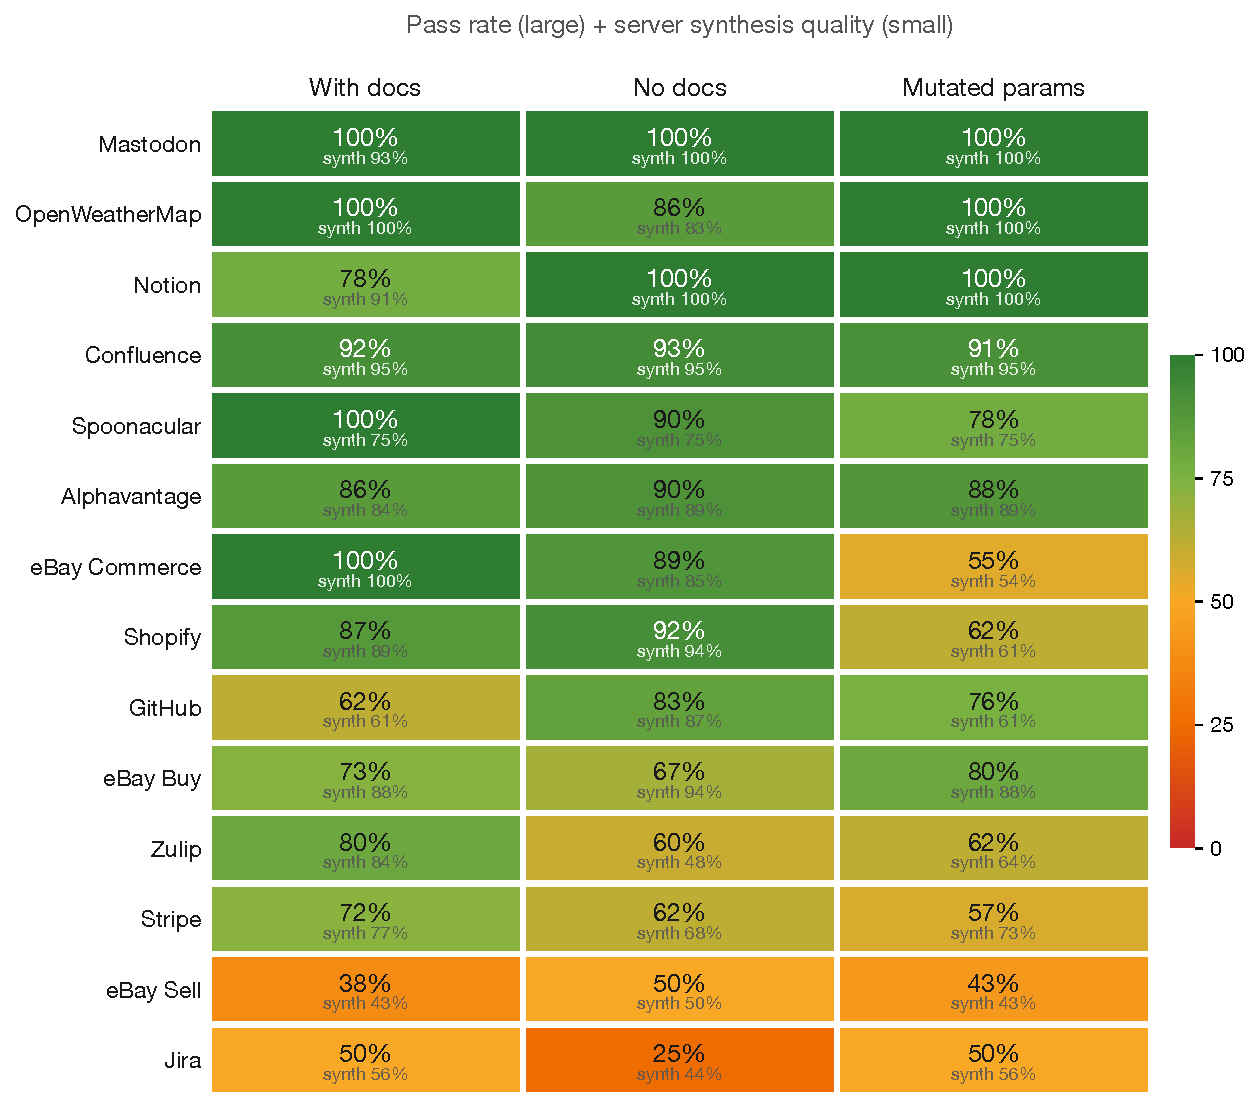
\includegraphics[width=\linewidth]{fig1_primary_heatmap.pdf}
  \caption{Agent pass rate (PASS, large) and server synthesis sufficiency
    (SYNTH, small) across 14 APIs and three synthesis conditions.
    Rows sorted by mean PASS descending.
    Colour encodes PASS on a red--orange--green scale.}
  \label{fig:heatmap}
\end{figure}

\begin{figure}[htbp]
  \centering
  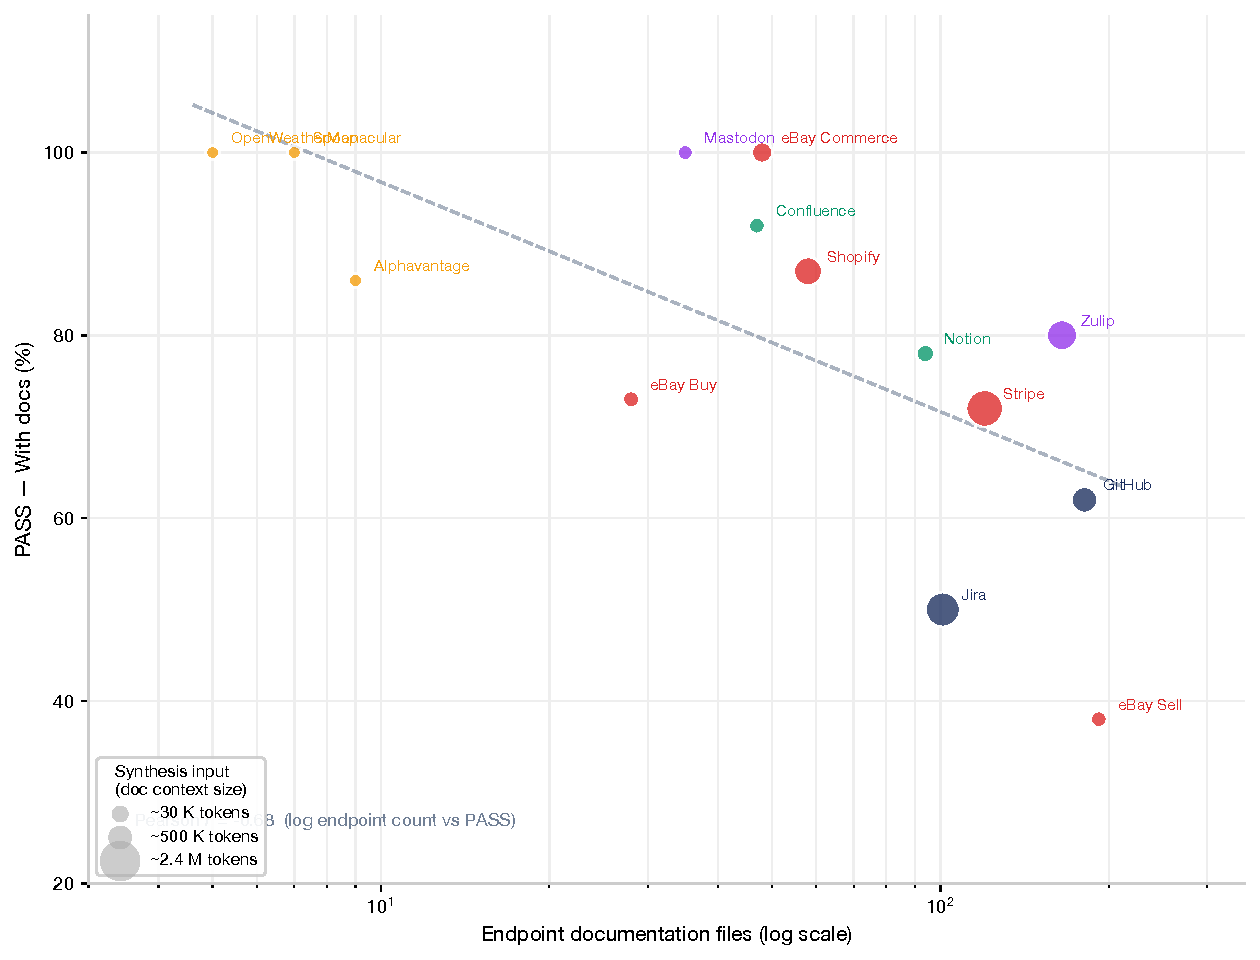
\includegraphics[width=0.72\linewidth]{fig8_api_complexity.pdf}
  \caption{API complexity (number of endpoint documentation files, log scale)
    vs.\ mean PASS in the docs condition. Larger APIs accumulate more
    coverage gaps, producing a negative trend between endpoint count and
    agent pass rate.}
  \label{fig:complexity}
\end{figure}

% ------------------------------------------------------------
\section{RQ2: Agent Task Completion}
\label{sec:rq2}
% ------------------------------------------------------------

\textbf{Do synthesized servers enable effective agent task completion,
compared to human-authored references?}

Figure~\ref{fig:strip} shows the distribution of PASS across APIs and
conditions. The median PASS is approximately 80\% in the docs condition and
85\% in the no-docs condition, with a long tail of high performers
(Mastodon 100\% across all three conditions; Confluence 91--93\%;
OpenWeatherMap 86--100\%) and a floor group (Jira mean 42\%;
eBay Sell mean 44\%; GitHub mean 55\% when the corrected mutated score is
included). The GitHub mean is suppressed primarily by the mutated condition
(19\%), which produces degenerate servers as detailed in
Section~\ref{sec:rq3}.

The variance across APIs is explained by two distinct mechanisms. For the
floor group, SYNTH is also low: Jira SYNTH=44--56\%, eBay Sell SYNTH=43\%.
These are synthesis failures masquerading as agent failures --- when the
required tools are absent, the agent cannot compensate. For APIs with
moderate PASS but higher SYNTH (Stripe: SYNTH=77\%, PASS=72\%), the
bottleneck shifts to agent reasoning on complex multi-step tasks: the
synthesis variance study reveals 8--14 AGENT\_REASONING undefined verdicts
per Stripe run, regardless of server coverage, indicating that the evaluation
agent fails on Stripe's multi-step invoice and subscription workflows
independently of tool availability. Figure~\ref{fig:scatter} makes this
distinction visible: points near the diagonal are synthesis-limited;
points well below it are agent-limited.

\begin{figure}[htbp]
  \centering
  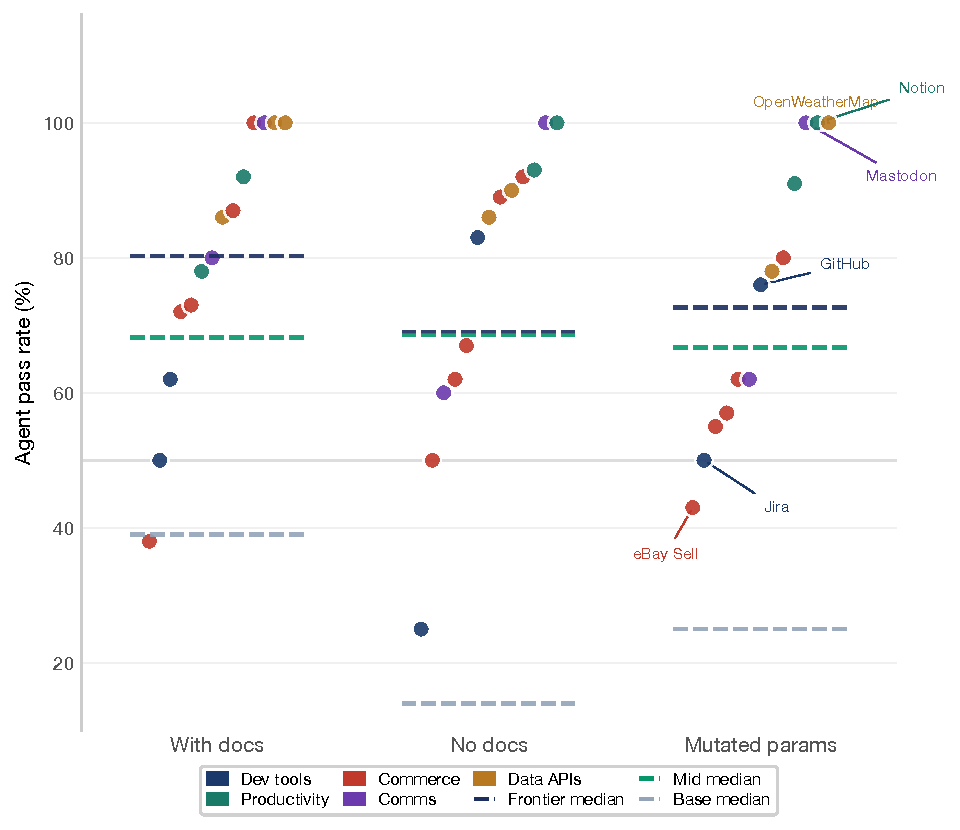
\includegraphics[width=0.85\linewidth]{fig2_condition_slopes.pdf}
  \caption{Distribution of PASS per synthesis condition.
    Each dot is one API; dashed line shows the median.
    The 50\% reference line is shown in light grey.}
  \label{fig:strip}
\end{figure}

\paragraph{Comparison with human-authored references.}
On GitHub, the community MCP server scores 65\% PASS. Synthesized servers
with docs match this (62--67\% across valid runs), and synthesized servers
without docs comfortably exceed it (83--90\%), because the synthesis model's
parametric knowledge of the GitHub API produces more complete tool coverage
than the hand-written reference. On Zulip, the community reference scores
68\%; the synthesized docs-condition server scores 80\%. In both cases the
human reference fails on the same \texttt{TOOL\_COVERAGE} pattern ---
missing webhooks, branch protection, and Actions dispatch for GitHub;
message edit, DM search, and scheduled messages for Zulip --- while the
synthesized server adds these endpoints.

% ------------------------------------------------------------
\section{RQ3: Parametric Knowledge and Documentation Faithfulness}
\label{sec:rq3}
% ------------------------------------------------------------

\textbf{To what extent do synthesizers rely on parametric knowledge rather
than documentation, and does this affect performance?}

The mutated-docs condition directly operationalises this question: if a
synthesizer adopts the renamed parameter names, it is reading the
documentation; if it does not, it is writing from memory.
Figure~\ref{fig:adherence} (left) shows mutation adherence rates across
APIs. GitHub, Stripe, Shopify, Zulip, and Jira all show near-zero HTTP
adoption --- the synthesis model completely ignores parameter mutations and
produces a server reflecting its training-time knowledge of the API.
Mastodon and Alphavantage exhibit full adoption (100\%), indicating the
synthesizer follows the provided documentation faithfully.

The right panel of Figure~\ref{fig:adherence} tests whether low adherence
predicts nodocs winning (the hypothesis being that strong parametric
knowledge makes documentation unnecessary or even harmful). The relationship
is weak and noisy. GitHub docs vs.\ nodocs fits the hypothesis: zero
adherence, nodocs wins by 21 percentage points (83\% vs.\ 62\%).
Stripe does not: also zero adherence, but docs still yield 10 percentage
points higher PASS (72\% vs.\ 62\%). This shows that parametric reliance at
the synthesis stage does not cleanly propagate to agent performance.

A more severe consequence of parametric reliance emerges in the mutated
condition for complex APIs. GitHub mutated PASS is only 19\% (SYNTH=22\%),
and the synthesis variance study shows 100\% degeneracy across seven
additional synthesis runs --- the mutated grounding document consistently
confuses the synthesizer, producing near-empty stubs of 0--6 tools against
GitHub's full API surface. This is a qualitatively different failure mode
from Shopify or Alphavantage mutated, where adherence is high and
synthesizers faithfully adopt renamed parameters: for those APIs,
documentation drives synthesis and mutations propagate cleanly into the
server. For GitHub, parametric gravity is so strong that any inconsistency
between the mutated document and training-time priors causes the synthesizer
to abort rather than reconcile --- resulting in structural failure rather than
wrong-name adoption.

The general mechanism is that the effect of parametric reliance depends on
whether the synthesis model and the evaluation agent share the same prior.
When both operate from training-time knowledge and the mutation context is
weak enough to be ignored (Stripe, Shopify), the pipeline is self-consistent
and performance matches the no-docs condition. When the mutated context is
strong enough to disrupt synthesis but not strong enough to guide it
completely (GitHub), degeneracy results. When adherence is high and the
evaluation agent lacks the same training-time prior, mutations propagate into
wrong API calls at the HTTP level.

\begin{figure}[htbp]
  \centering
  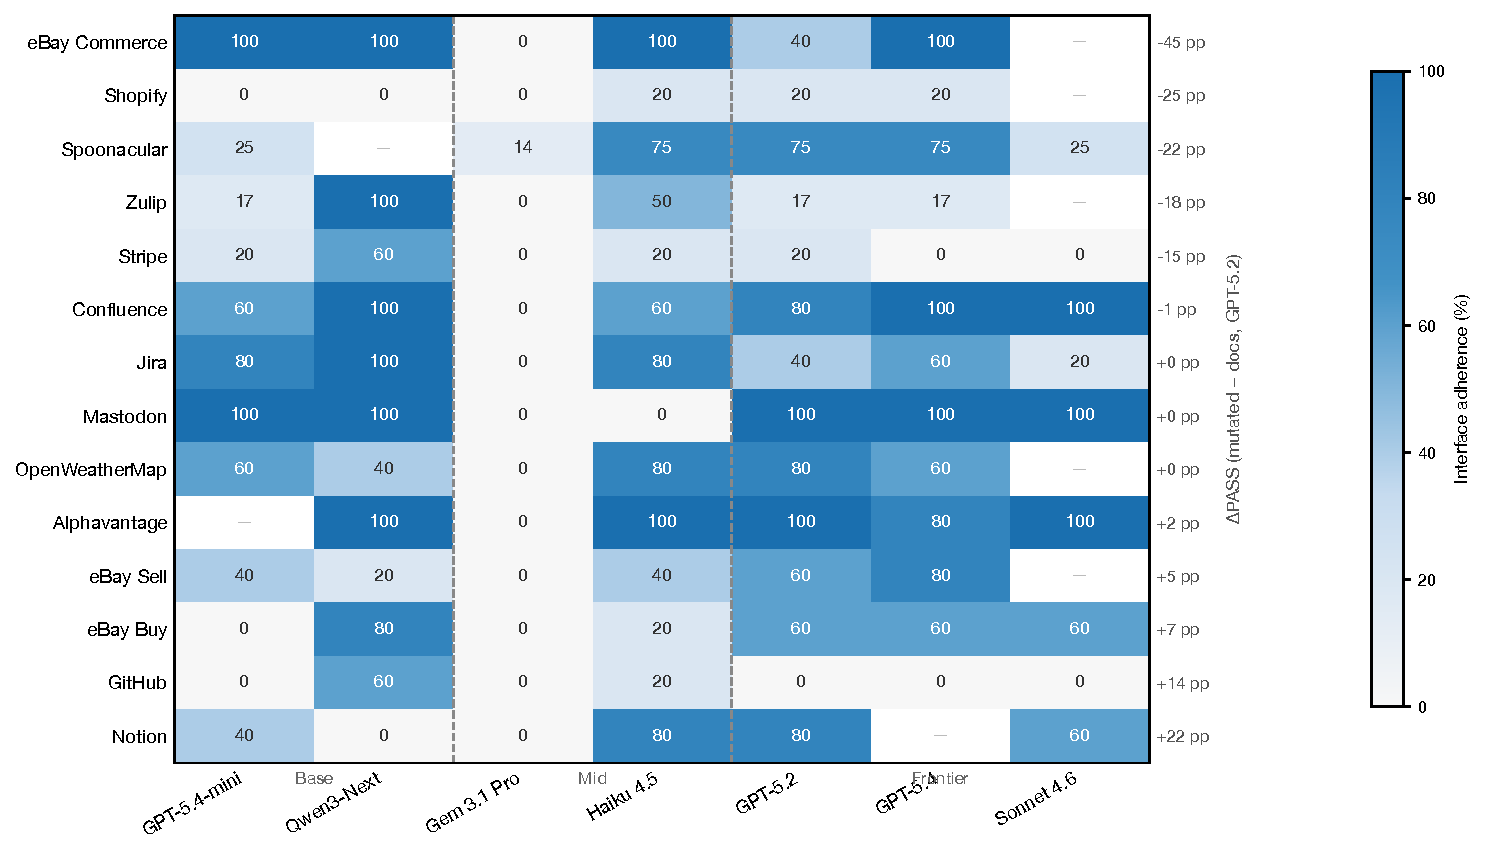
\includegraphics[width=\linewidth]{fig6_mutation_sensitivity.pdf}
  \caption{Mutation sensitivity and adherence. Left: per-API PASS delta
    (docs minus mutated), showing which APIs are most sensitive to
    parameter renaming. Right: HTTP mutation adherence rate per API,
    sorted by HTTP adoption. Zero HTTP adherence indicates the synthesizer
    relied on parametric knowledge rather than the mutated documentation.}
  \label{fig:adherence}
\end{figure}

% ------------------------------------------------------------
\section{RQ4: Effect of Documentation Availability}
\label{sec:rq4}
% ------------------------------------------------------------

\textbf{How does documentation availability affect synthesis and agent
performance?}

Figure~\ref{fig:strip} shows the median PASS per condition. The no-docs
median (85\%) closely matches the docs median (80\%), indicating that
removing documentation does not on average degrade agent performance.
This aggregate result conceals meaningful per-API variation, visible in
Figure~\ref{fig:docs_effect}.

\begin{figure}[htbp]
  \centering
  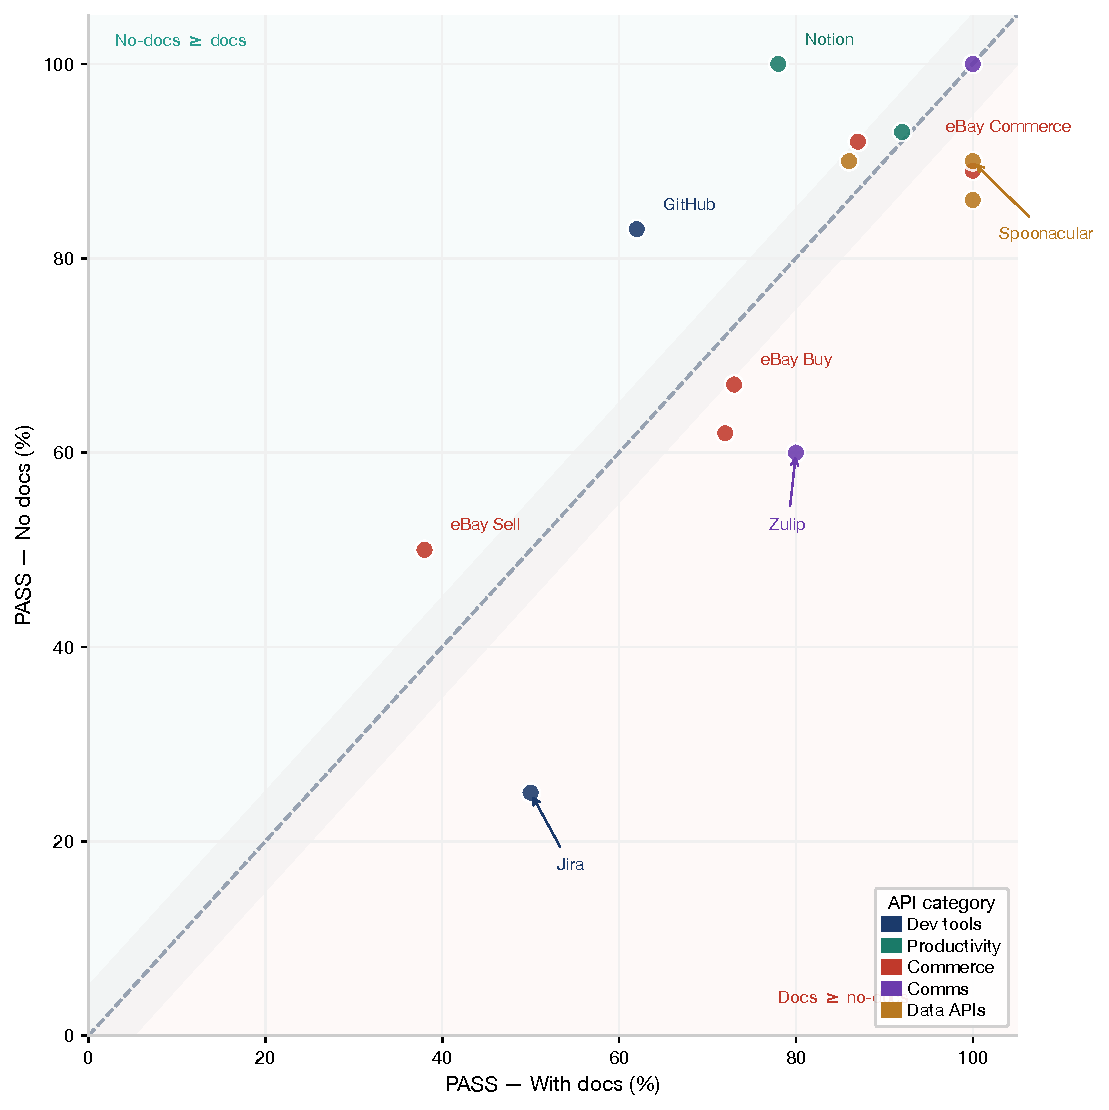
\includegraphics[width=0.72\linewidth]{fig7_docs_effect.pdf}
  \caption{Docs vs.\ no-docs PASS per API. Points above the diagonal
    indicate APIs where removing documentation improved performance;
    points below indicate APIs where documentation helped.}
  \label{fig:docs_effect}
\end{figure}

APIs above the diagonal (nodocs wins) include GitHub, Notion, and Mastodon:
high-frequency, well-documented APIs for which the synthesis model has
strong training-time priors. Removing documentation reduces noise and allows
the model to produce a clean, complete server from memory. APIs below the
diagonal (docs help) include Stripe and Zulip: less saturated in training
data, or with API conventions sufficiently idiosyncratic that documentation
provides genuine signal the model could not otherwise recover.

The mutated condition (also visible in Figure~\ref{fig:strip}) shows a
further decrease in the median (approximately 70\%), indicating that
parameter renaming introduces meaningful aggregate degradation.
The most extreme case is GitHub mutated: corrected re-evaluation scores
only 19\% PASS (SYNTH=22\%), compared to 62\% (docs) and 83\% (nodocs).
This collapse is driven not by parameter adoption failures but by synthesis
degeneracy --- the mutated grounding document causes the synthesizer to
produce near-empty stubs, so the agent has almost no tools to work with.
For APIs where adherence is high (Mastodon, Alphavantage), mutations
propagate cleanly and the mutated server scores near the docs baseline.
The harm from mutations is thus mediated by whether the synthesizer adopts
them (adherence-limited) or by whether the mutated context disrupts synthesis
entirely (degeneracy-limited).

% ------------------------------------------------------------
\subsection{Synthesis Model Comparison}
\label{sec:synth-models}
% ------------------------------------------------------------

Figure~\ref{fig:model-comp} compares four synthesis models on GitHub, Stripe,
and Zulip across all three conditions. The primary baseline (GPT-5.2) scores
62--80\% across these datasets in the docs condition. Sonnet~4.6 substantially
outperforms GPT-5.2 on GitHub (90\%/100\%/100\% docs/nodocs/mutated) and
Stripe (77\%/100\%/100\%), demonstrating that context adherence --- measured
by mutation adoption in RQ3 --- translates to downstream gains when the
model genuinely reads the provided documentation. GPT-5.4 shows a
catastrophic regression on Stripe docs (8\% vs.\ 72\% for GPT-5.2), caused
by incorrect HTTP method mapping in synthesized stubs --- a reminder that
newer models can exhibit novel failure modes on API integration tasks.
Qwen3-Coder-Next produces structural failures (crash or no \texttt{server.py})
on Zulip docs and nodocs, indicating that smaller or less instruction-tuned
models have a higher floor for this task.

\begin{figure}[htbp]
  \centering
  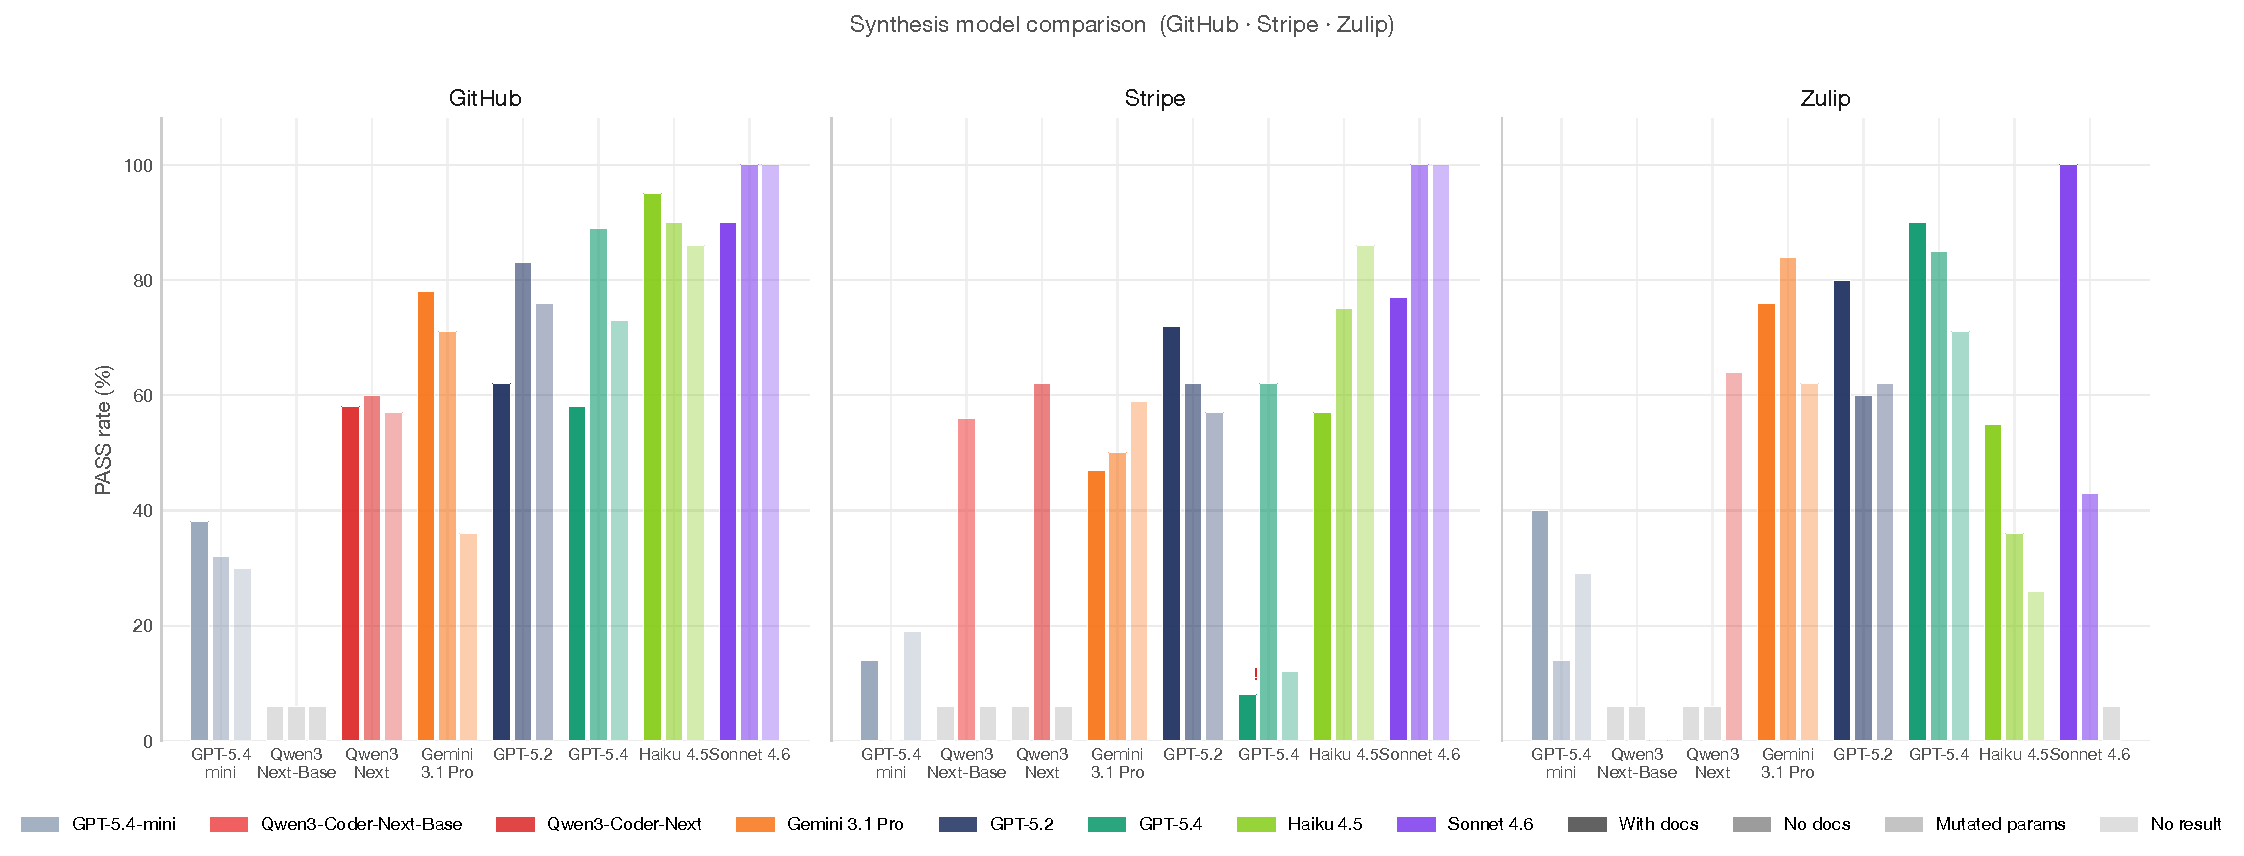
\includegraphics[width=\linewidth]{fig3_model_comparison.pdf}
  \caption{Synthesis model comparison on GitHub, Stripe, and Zulip
    across three conditions. Hatched bars indicate synthesis failure
    (crash or no evaluable server). GPT-5.4 Stripe docs (8\%) is
    a catastrophic regression relative to the GPT-5.2 baseline (72\%).}
  \label{fig:model-comp}
\end{figure}

% ------------------------------------------------------------
\section{RQ5: Synthesis Quality as a Predictor of Agent Performance}
\label{sec:rq5}
% ------------------------------------------------------------

\textbf{Does synthesis quality predict agent task performance?}

Figure~\ref{fig:scatter} plots SYNTH against PASS for all 42 API--condition
pairs. The Pearson correlation is $r = 0.921$ ($p < 0.0001$, $n = 42$),
indicating a strong linear relationship between synthesis sufficiency and
agent pass rate. This is the central methodological validation result: SYNTH
is a reliable proxy for downstream utility, and failures in synthesis
propagate to agent failures with high fidelity.

\begin{figure}[htbp]
  \centering
  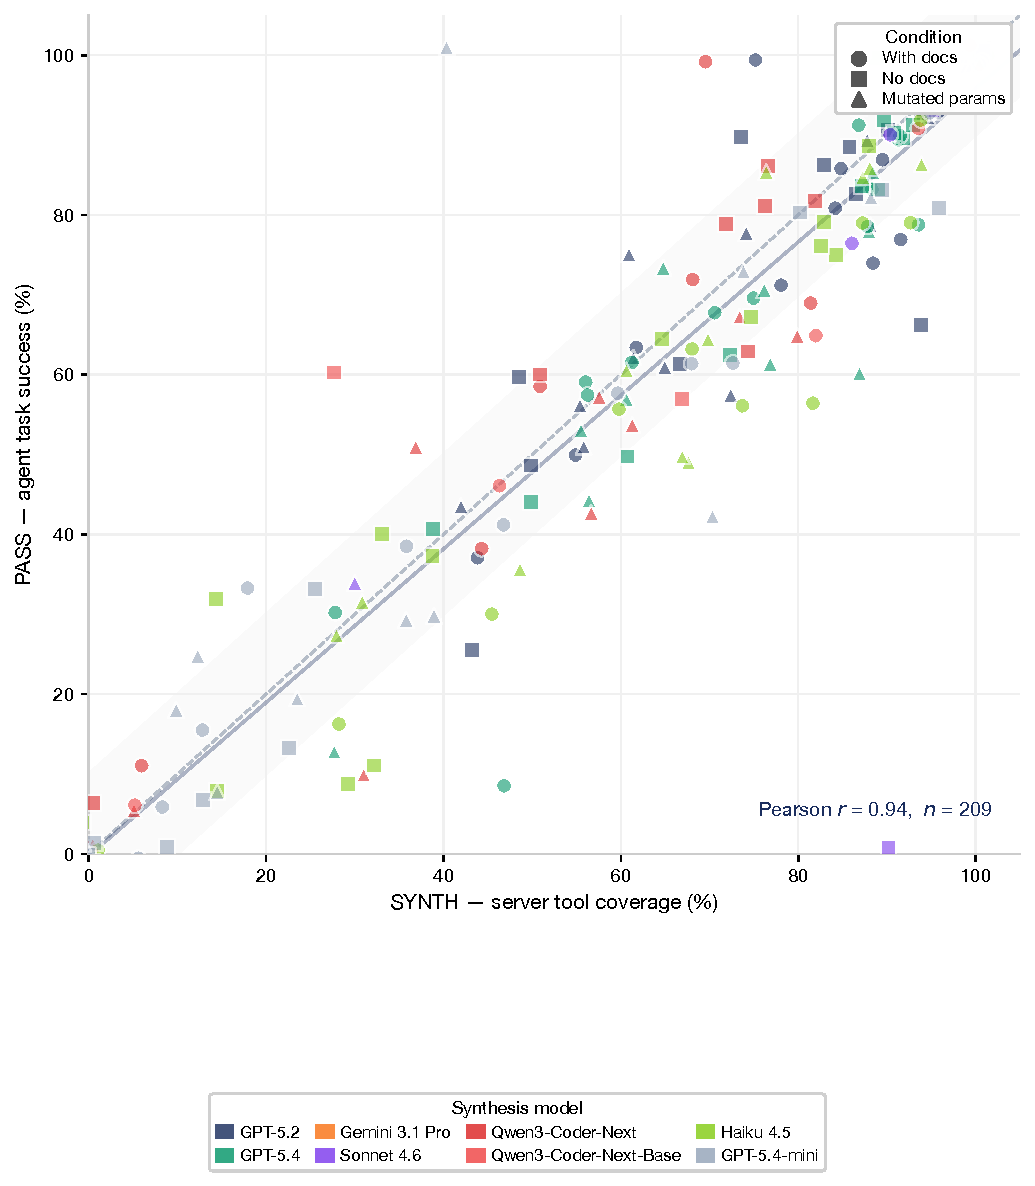
\includegraphics[width=0.72\linewidth]{fig4_synth_scatter.pdf}
  \caption{SYNTH vs.\ PASS across all 42 API--condition pairs
    ($r \approx 0.92$). Shape encodes synthesis condition;
    colour encodes API category.
    The dashed line is $y = x$; the grey band is $\pm 10$ pp.}
  \label{fig:scatter}
\end{figure}

The points near or above the diagonal represent cases where the agent
performs at or above what synthesis quality would predict --- most commonly
when the agent compensates for minor coverage gaps with general reasoning
(Spoonacular: SYNTH=75\%, PASS=100\% in the docs condition). Points well
below the diagonal (eBay Commerce mutated: SYNTH=54\%, PASS=55\%) confirm
that when synthesis fails to cover the task space, agent performance cannot
recover. The Jira no-docs outlier (SYNTH=44\%, PASS=25\%) represents the
most severe case of synthesis-induced failure in the benchmark.
The corrected GitHub mutated point (SYNTH=22\%, PASS=19\%) lies
near the diagonal, confirming that when synthesis degeneracy is
acknowledged, SYNTH and PASS align closely.

Taken together, these results validate SYNTH as a leading indicator:
measuring synthesis sufficiency before running the full evaluation pipeline
gives a reliable estimate of whether agent task completion will succeed.

% ============================================================
\chapter{Discussion}
\label{ch:discussion}
% ============================================================

\section{Synthesis as a General Capability}

The central empirical finding is that LLM-based tool synthesis is broadly
feasible: twelve of fourteen APIs achieve SYNTH $\geq 75\%$ under the
best synthesis condition, and the median agent pass rate of 80\% demonstrates
that synthesized servers are not merely structurally valid but functionally
useful. This is a non-trivial result. REST API integration involves strict
interface contracts, multi-step authentication flows, and domain-specific
parameter conventions --- constraints that probabilistic generation does not
inherently respect. That synthesis models navigate these requirements reliably
across domains as diverse as e-commerce, communication, and financial data
suggests the capability is not narrow or brittle.

The two failure cases --- Jira and eBay Sell --- share a structural
characteristic: extremely large documentation corpora with hundreds of
endpoints distributed across deeply nested resource hierarchies. This points
to a \emph{coverage scaling problem} rather than a fundamental inability to
synthesize: the model understands the API but cannot attend to all endpoints
within a single synthesis context. This is consistent with findings on
positional bias in long contexts~\cite{liu2023lostmiddle,disentanglerecall2025},
and suggests that decomposition strategies --- synthesizing one API resource
group at a time and assembling the results --- could close this gap without
requiring larger context windows.

The comparison with human-authored reference servers on GitHub and Zulip
sharpens this conclusion. Synthesized servers match the GitHub community
server in the docs condition and substantially exceed it without documentation,
while exceeding the Zulip reference in both conditions. The human references
fail consistently on the same pattern: they cover the core, frequently-used
API surface but omit less common but task-relevant endpoints (webhooks and
Actions dispatch for GitHub; message edit and DM search for Zulip). A
synthesis agent, by contrast, reads the full documentation and attempts
comprehensive coverage --- and because it is not resource-constrained in the
way a human contributor might be, this breadth comes without a corresponding
quality trade-off.

\section{Parametric Gravity: Mechanism and Consequence}

The mutation adherence results reveal a sharp split across APIs.
High-familiarity APIs (GitHub, Stripe, Shopify, Zulip, Jira) exhibit
near-zero HTTP-layer adherence: the synthesis model ignores parameter
mutations entirely and produces servers that reflect its training-time
knowledge of the API. Low-familiarity APIs (Mastodon, Alphavantage) show
near-complete adherence. This binary pattern is consistent with
the training-frequency hypothesis of Mallen et al.~\cite{mallen2023knowns}:
entities well-represented in pre-training data are retrieved from weights
rather than from context.

The consequence for downstream performance is, however, more nuanced than a
simple ``parametric reliance hurts'' narrative. For GitHub, zero adherence
coincides with the highest PASS gains in the no-docs condition (+21 pp): the
model writes from memory, and its memory is accurate. For Stripe, zero
adherence coincides with a \emph{docs advantage} (+10 pp): the model also
writes from memory, but documentation provides additional signal that
improves coverage. The mechanism that determines which outcome obtains is
whether the synthesis model's training-time representation of the API is
complete enough to be relied upon. GitHub's API, being one of the most
heavily documented REST APIs on the web, almost certainly saturates model
memory. Stripe's is large and has evolved significantly since the likely
training cutoff of the primary models --- a scenario identified by
Lagging~\cite{lagging2025} as particularly susceptible to silent
faithfulness failures.

This interpretation has a practical implication: whether to include
documentation in the synthesis context is not a universal design choice but
an API-specific one, and the right decision correlates with how confidently
the synthesis model can write from memory. A pre-synthesis probe --- for
example, asking the model to generate a list of API endpoints before
providing documentation --- could serve as a low-cost signal for this
confidence.

\section{Representational Dynamics: Preliminary Probing Evidence}

The behavioural adherence results raise a mechanistic question: at which
layer in the forward pass does parametric gravity assert itself? If a model
ignores a mutated parameter name despite it being present in the context,
the in-context representation must at some layer be overridden by a
training-time attractor --- a pattern that prior mechanistic work localises
to middle-layer feed-forward modules~\cite{meng2022rome,factualrecall2025}.

Our preliminary log-linear probing analysis on a smaller open-weight model
provides a first empirical window into this. Probing the residual stream at
each transformer layer for whether the mutated or original parameter name is
better predicted reveals a characteristic transition: early layers
faithfully represent the in-context token (high probe accuracy for the
mutated name), while mid-to-late layers shift toward the training-time
prior (high probe accuracy for the original name). This transition layer
varies by API: it occurs earlier for high-familiarity APIs (GitHub-like)
than for low-familiarity ones (Mastodon-like), consistent with stronger
parametric attractors for APIs more densely represented in training data.

These findings align with recent work on how post-training reshapes
representations~\cite{posttrainingreshapes2025}: instruction fine-tuning
and RLHF alter the geometry of the residual stream in ways that could
modulate the transition point. This suggests that the choice of synthesis
model --- not just pre-training corpus composition but also fine-tuning
regime --- affects the layer at which context is overridden. It also
identifies a concrete intervention point: a targeted context-faithful
fine-tuning signal applied at the transition layers could, in principle,
reduce parametric gravity without sacrificing the broader capabilities that
make these models effective synthesizers.

This analysis is exploratory; results are on a single smaller model and
should not be over-generalised. We include it to ground the behavioural
patterns in an emerging mechanistic framework and to motivate future work
connecting probing methodology to the synthesis setting.

\section{Synthesis Quality as a Proxy Metric}

The strong SYNTH--PASS correlation ($r = 0.921$, $p < 0.0001$, $n = 42$)
has a direct practical implication: synthesis sufficiency, assessed by an
LLM judge examining the server's tool list without running the evaluation
agent, is a reliable predictor of downstream agent task performance. This
matters because the full evaluation pipeline --- spinning up a sandboxed API
environment, running the evaluation agent for up to 15 turns per task,
calling the judge --- is expensive in both API quota and wall time. SYNTH
can be assessed at synthesis time, before any agent evaluation occurs.

The two regimes visible in Figure~\ref{fig:scatter} sharpen when this
metric is used diagnostically. For synthesis-limited cases (low SYNTH, low
PASS), investment in improving synthesis quality --- better documentation
pre-processing, larger context windows, iterative tool refinement --- will
directly improve agent outcomes. For agent-limited cases (high SYNTH, lower
PASS), the bottleneck is the evaluation agent's ability to compose available
tools into correct multi-step plans, and improving synthesis will not help;
the intervention should target the agent's reasoning or task decomposition.

One class of outlier is worth noting: Spoonacular in the docs condition
achieves PASS=100\% despite SYNTH=75\%. This occurs because the evaluation
agent compensates for minor coverage gaps using general culinary knowledge
to reformulate queries through available tools. This agent-compensation
effect is bounded --- it requires the agent to have its own parametric
knowledge about the domain --- and cannot be relied upon for APIs in
unfamiliar domains (compare Jira, where the agent has no comparable domain
model to fall back on).

\section{Practical Design Guidelines}

The results point to several concrete recommendations for practitioners
building LLM-based tool synthesis systems.

\paragraph{Documentation pre-processing matters for large APIs.}
For APIs with more than approximately 50 endpoints, raw documentation dumps
produce coverage gaps: the synthesizer cannot attend to all endpoints in a
single pass. Structured chunking by resource group, with per-chunk synthesis
followed by assembly, is likely to produce higher SYNTH scores than
end-to-end synthesis from a monolithic documentation corpus.

\paragraph{Omitting documentation is safe for high-familiarity APIs.}
For APIs heavily represented in model training data --- GitHub, Stripe,
major productivity platforms --- the no-docs condition matches or exceeds
the docs condition. Documentation can add noise by providing competing
context that the model must adjudicate against its priors, particularly
for long, partially-outdated documentation files. Practitioners should
consider a pre-synthesis familiarity check before deciding whether to
include documentation in the synthesis context.

\paragraph{Grounding manifests provide a weak but useful quality signal.}
Requiring the synthesizer to produce a \texttt{grounding.json} enables a
fast post-synthesis check: verify that every tool is anchored to an existing
documentation file and a syntactically valid endpoint string. This does not
guarantee implementation correctness --- a model can cite the right document
while misreading it --- but tools lacking any documentation anchor are a
reliable signal of unconstrained parametric generation, and missing grounding
coverage (tools with no entry) often correlates with structural synthesis
failures.

\paragraph{SYNTH is a cheap pre-flight metric.}
Running an LLM judge over the tool list before committing to full agent
evaluation identifies synthesis-limited cases early. A SYNTH threshold
of around 75\% appears to be the boundary below which full evaluation
is unlikely to produce acceptable PASS rates in our benchmark; APIs
below this threshold benefit more from re-synthesis than from agent
tuning.

\paragraph{Prefer models with strong context-faithfulness for mutating or
evolving APIs.}
When the target API is less familiar to the model, or when documentation
has been deliberately structured to override training priors (as in our
mutated condition), synthesis models that exhibit higher context adherence
--- Sonnet~4.6 in our comparison --- produce more reliable servers. The
GPT-5.4 regression on Stripe (8\% vs.\ 72\% baseline) illustrates the risk
of deploying a model with strong parametric priors on an API that has
evolved since its training cutoff.

\section{Comparison with Prior Work}

Direct numerical comparison with prior work is complicated by the absence of
overlapping evaluation sets: ToolFactory~\cite{toolfactory2025} and
Doc2Agent~\cite{doc2agent2025} each evaluate on their own API selections
and do not report PASS rates on the same 14 APIs used here. Qualitative
comparison is nonetheless informative.

ToolFactory targets OpenAPI-specified inputs and focuses on coverage of the
formal schema; our benchmark uses raw Markdown documentation, a substantially
harder input modality that better reflects real practitioner conditions. Where
ToolFactory reports synthesis success in terms of schema coverage, we report
end-to-end agent task completion, which additionally exercises tool naming,
description quality, and implementation correctness under live API execution.

Doc2Agent is closest to our work in motivation: it demonstrates that MCP
servers can be generated from documentation at scale across many APIs. Our
benchmark adds the no-docs and mutated conditions that Doc2Agent does not
evaluate, enabling the parametric knowledge analysis that is our primary
empirical contribution. Doc2Agent also does not measure whether synthesized
servers match or exceed human-authored alternatives; our comparison against
the GitHub and Zulip community servers provides evidence on that question.

WAPIIBench~\cite{wapiibench2025} catalogues LLM-generated API integration
errors against live services and reports error taxonomies that partially
overlap with our failure cause categories (\textsc{tool\_schema},
\textsc{tool\_implementation}). Their finding that authentication and
parameter serialisation errors are the most frequent failure types is
consistent with our observation that synthesis failures are more often
coverage gaps than implementation bugs in the tools that \emph{are} produced.

\section{Limitations}

\paragraph{Generalizability.}
The 14-API evaluation set spans five domains and a wide range of API sizes,
but is not exhaustive. All selected APIs are REST-based, return JSON, and
have English-language documentation. APIs with non-REST interfaces (GraphQL,
gRPC), streaming responses, complex webhook architectures, or non-English
documentation are not represented. The degree to which the parametric gravity
findings generalise to programming-language SDKs rather than HTTP APIs is
also unknown: the mutation adherence analysis is specific to the HTTP
parameter-name setting.

\paragraph{Reliability.}
PASS rates are determined by an LLM judge, which introduces variability.
We use a fixed judge model (Gemini~3~Flash) with a structured fixed-format
prompt to reduce inconsistency, but judge agreement with human annotation
has not been formally validated for this benchmark. Similarly, the
probing analysis rests on a single open-weight model; results should not
be taken as established fact about frontier-scale models.

\paragraph{Reproducibility.}
All synthesis runs are stochastic: the same synthesis model and documentation
may produce a different server on a different run. We report single-run
results per condition rather than averages over multiple runs, which means
some variance in PASS and SYNTH is unaccounted for. API sandboxes may also
change state between runs, introducing noise in write-task evaluations.

\paragraph{Ethical considerations.}
Automated tool synthesis lowers the barrier to creating API integrations,
including potentially for APIs whose terms of service restrict automated
access or data extraction. The benchmark deliberately uses official sandbox
environments with test credentials, but production deployment of synthesis
pipelines against APIs not designed for automated access raises ToS and
privacy concerns that practitioners should assess case by case. There is
also an energy cost to running large synthesis models at scale; the
no-docs condition, which is substantially cheaper, may be preferable
where API familiarity is high, reducing unnecessary compute.

% ============================================================
\chapter{Conclusion}
\label{ch:conclusion}
% ============================================================

This thesis addressed a gap in the tool-use literature: the assumption that
tools are given. We asked whether language models can synthesize functional
API tool servers from documentation, whether those servers enable effective
agent task completion, and what role parametric knowledge plays in both.
Below we answer each research question and qualify the answers with the
relevant limitations of the study.

\paragraph{RQ1: Can LLMs synthesize functional API tool servers from
documentation alone?}
Yes, for most APIs tested. Twelve of fourteen APIs achieve SYNTH $\geq 75\%$
in the docs condition, and the dominant failure mode is coverage gap (omitted
endpoints) rather than structural failure (broken or non-executable servers).
This answer is qualified by generalizability: all APIs in the benchmark are
REST-based with English documentation, and synthesis feasibility for larger
or differently structured APIs remains to be established. Single-run
evaluation also means some variance in these figures is unaccounted for.

\paragraph{RQ2: Do synthesized servers enable effective agent task completion,
compared to human-authored references?}
Yes, at a median PASS of 80\% in the docs condition, and synthesized servers
match or exceed the two available human-authored references. On GitHub,
no-docs synthesis achieves 83--90\% PASS against a community server baseline
of 65\%; on Zulip, docs-condition synthesis scores 80\% against a baseline
of 68\%. The qualification here is that agent performance is partially
confounded by the fixed evaluation agent (Gemini~2.5~Pro); agent-limited
failures identified in our benchmark may not reflect the same limitations
with a different evaluator.

\paragraph{RQ3: To what extent do synthesizers rely on parametric knowledge,
and does this affect performance?}
Substantially, and in a way that is API-dependent. High-familiarity APIs
show near-zero HTTP mutation adherence, indicating synthesis models write
almost entirely from memory. The performance consequence is non-monotonic:
parametric reliance helps on GitHub (where model memory is accurate and
complete) but does not on Stripe (where documentation provides additional
coverage). This answer is limited by the fact that adherence is measured
only for the primary synthesis model (GPT-5.2) and for a fixed set of
4--6 mutated parameters per API; the pattern may differ for other models
or mutation strategies.

\paragraph{RQ4: How does documentation availability affect synthesis and
agent performance?}
The aggregate effect is smaller than expected: the no-docs condition median
(85\%) closely matches the docs condition median (80\%), driven by
high-familiarity APIs where model memory substitutes for documentation.
Documentation helps for less familiar APIs (Stripe, Zulip) and hurts for
highly familiar ones (GitHub, Mastodon), suggesting the effect is mediated
by training coverage rather than documentation quality per se. This finding
is subject to the static-snapshot limitation: documentation was scraped at
a single point in time, and results may differ for documentation that is
more consistently current.

\paragraph{RQ5: Does synthesis quality predict agent task performance?}
Strongly: $r = 0.921$ ($p < 0.0001$, $n = 42$). SYNTH, assessable without
running the evaluation agent, is a reliable proxy for PASS. This holds
across APIs and conditions, with the main exceptions being cases where the
evaluation agent compensates for synthesis gaps using its own domain
knowledge (Spoonacular) or where the agent fails despite sufficient tools
(agent-limited cases). The correlation is measured on our 14-API benchmark;
whether it holds at this strength for a wider or different API distribution
is unknown.

\section*{Research Gap and Contribution}

Prior work treats the tool layer as given. We have shown that synthesizing
it automatically is feasible today for most practically relevant REST APIs,
and that the primary bottleneck for large APIs is context-window coverage
of documentation rather than a fundamental capability limit. The SYNTH
metric and the controlled ablation design --- isolating parametric knowledge
from documentation grounding --- are methodological contributions that
generalise beyond this benchmark to any evaluation of documentation-grounded
code generation.

\section*{Future Work}

The coverage scaling problem for large APIs (Jira, eBay Sell) is the most
direct target for follow-on work: decomposed synthesis by resource group,
with per-chunk synthesis and assembly, is a natural approach the current
benchmark motivates but cannot evaluate. A multi-agent evaluation sweep
would disentangle synthesis quality from evaluation-agent-specific reasoning.
Extending the probing analysis to frontier-scale open-weight models would
test whether the layer-transition pattern is general. Finally, a live
benchmark that re-runs synthesis as APIs evolve would capture the dynamic
challenge that static snapshots cannot.

\bibliographystyle{plain}
\bibliography{thesis-ai-template/bibentries}

\end{document}
